\documentclass[times, utf8, proizvoljni, numeric]{fer}

\usepackage{booktabs}
\usepackage{amsmath}
\usepackage{nccmath}
\usepackage{hyperref}
\usepackage[section]{placeins}
\usepackage{indentfirst}

\usepackage{footnote}
\usepackage{graphicx}
\usepackage{float}
\usepackage{mathtools}
\usepackage{makecell}
%\usepackage[hidelinks]{hyperref}
\usepackage{subcaption,graphicx}

\renewcommand\theadalign{cb}
\renewcommand\theadfont{\bfseries}
\renewcommand\theadgape{\Gape[4pt]}
\renewcommand\cellgape{\Gape[4pt]}

\DeclarePairedDelimiter\ceil{\lceil}{\rceil}
\DeclarePairedDelimiter\floor{\lfloor}{\rfloor}

\DeclareMathOperator*{\argmin}{\arg\!\min}
\DeclareMathOperator*{\argmax}{\arg\!\max}

\newcommand{\rulesep}{\unskip\ \vrule\ }

% Hyperref setup
\hypersetup{
	colorlinks=true,
	linkcolor=black,
	filecolor=magenta,      
	urlcolor=cyan,
}
\urlstyle{same}
%

\begin{document}


\title{Ekstrahiranje značajki slika pomoću dubokog učenja u svrhu poboljšanja sustava preporuke slika}
\author{Toni Vlaić, Viran Ribić}

\maketitle

% Ispis stranice s napomenom o umetanju izvornika rada. Uklonite naredbu \izvornik ako želite izbaciti tu stranicu.
% Dodavanje zahvale ili prazne stranice. Ako ne želite dodati zahvalu, naredbu ostavite radi prazne stranice.
\thispagestyle{empty}
\zahvala{\begin{center}Ovaj rad izrađen je u Zavodu za elektroniku, mikroelektroniku, računalne i inteligentne sustave Fakulteta elektrotehnike i računarstva Sveučilišta u Zagrebu pod vodstvom doc. dr. sc. Marina Šilića i predan je na natječaj za dodjelu Rektorove nagrade u akademskoj godini 2017./2018.
		\end{center}
}

\tableofcontents
\thispagestyle{empty}
\listoftables
\thispagestyle{empty}
\listoffigures
\thispagestyle{empty}
%%%%%%%%%%%%%%%%%%%%%%%%%%%%%%%%%%%%%%%%%%%%%%%%%%%%%%%%%%%%%%%%%%%%%%%%%%%%%%%%%%%%%%%


%% CHAPTER
\chapter{Uvod}


Digitalne slike čine jedinstveni format kojim se može opisati veliki broj različitih informacija o stvarnom svijetu. Sadržaj slike može uključivati tekstualne dokumente, satelitske snimke, medicinske zapise, ljudske interakcije, promet na cestama ili u zraku. Navedene su samo neke od kategorija od interesa koje možemo zabilježiti u digitalnom formatu, zajednički za sve interpretacije. Trodimenzionalni matrični zapis u računalu može opisati ogroman broj pojava koje susrećemo u stvarnom svijetu. Sve informacije koje čovjek razlučuje kroz vid mogu biti predstavljene u računalu u obliku informacije o intenzitetu svjetlosti i odnosu među susjednim pikselima. Reprodukcija ljudskog vizualnog sustava nije trivijalna, ali pruža alternativni pogled na računalne sustave inspirirane biološkim sustavima. Dva nova trenda u računarstvu su posljednjih godina potaknula velik broj istraživanja na području analize slike: enormne količine podataka koje se generiraju u svijetu i napredak u oblikovanju inteligentnih sustava i umjetne inteligencije. 

Danas slike čine veliki udio podataka na internetu. Dok je egzaktna informacija o postotku slika na internetu intraktabilna, provedene analize iz 2016. godine \cite{img-analysis} predviđale su porast od trilijun slika u narednoj godini. Rast slikovnih podataka povezan je s brojem korisnika pametnih telefona u svijetu kao i brojem online usluga koje uključuju obradu i razmjenu fotografija. Rastući trendovi korisnika \cite{net-users} i napreci u telekomunikacijskim tehnologijama omogućuju lakšu i bržu distribuciju medijskih datoteka nego ikad prije. 

Volumen i protok podataka u današnjim sustavima učinio je bilo kakvu ručnu obradu slika neadekvatnom što je potaknulo istraživače na razmatranje novih metoda pri analizi velikih količina podataka. Da bi se podacima moglo upravljati potrebno je prvo razviti efikasne metode pretrage. Novonastala situacija pronalazi sličnosti s ranim danima interneta dok još nisu formirane adekvatne metode pretraživanja stranica. Izmjena informacija bila je znatno teža zbog nedostatka prikladnih sučelja koja bi običnim korisnicima mogla pružiti jednostavno korištenje. Tek su se pojavom algoritama za indeksiranje otvorile sve mogućnosti izmjene podataka na internetu. Izgradnjom adekvatnih algoritama za pretraživanje i ekstrakciju znanja postići ćemo bolje razumijevanje podataka i omogućiti njihovu efikasniju upotrebu. 

Ben Silbermann, osnivač i direktor društvene mreže Pinterest, izjavio je kako će budućnost internet pretraživača biti upravo u efikasnoj interpretaciji slika. Za razliku od današnjih internetskih pretraživača koje se prvenstveno oslanjaju na ključne riječi unutar stranice, takvi bi pretraživači bili sposobni razumjeti semantiku slike i izvaditi ključne koncepte povezane s upitima korisnika \cite{internet-trends}.

Društvene mreže samo su jedan od primjera gdje će razumijevanje semantike slika imati ključnu ulogu u narednim godinama. Potražnja za ekstrakcijom znanja iz slika primjetna je i u marketinškim \cite{electronic-commerce-application}, medicinskim \cite{medical-application} \cite{medical-diagnostics-application}, državnim \cite{smart-city-application}, sigurnosnim \cite{security-application} i forenzičkim \cite{forensics-application} primjenama. 

Napredak sklopovlja vratio je u fokus modele neuronskih mreža pošto su nove arhitekture grafičkih kartica bile dovoljno efikasne za ponovno eksperimentiranje s umjetnim neuronskim mrežama. Rezultat novog vala testiranja bile su dublje mreže, sposobne uhvatiti kompleksnije odnose među pikselima slika čime je označen početak dubokog učenja. Prikupljeni podaci o slikama sada postaju predmet proučavanja ovih pametnih algoritama koji pronalaze nove primjene u akademiji i industriji. 

Ovaj rad proučava postojeće arhitekture i modele dubokog učenja i istražuje njihove primjene u oblikovanju sustava preporuke slika ekstrakcijom njihovih značajki. U nastavku uvodnog poglavlja rada izlažu se opći i specifični ciljevi te programski paketi korišteni u implementaciji. Drugo poglavlje obrađuje modele za sažimanje opisujući arhitekturu dubokih konvolucijskih mreža i predtreniranih modela \textit{VGG} i \textit{Inception v4}. Također, u poglavlje je uključen opis algoritma analize glavnih komponenti koji je korišten za efikasniju reprezentaciju značajki. Slijedi ih odjeljak s rezultatima i raspravom o ispitanim metrikama sličnosti, ponašanju predtreniranih arhitektura i metodama za inspekciju kvalitete modela na našem zadatku. Četvrto poglavlje pokriva demonstraciju rada sustava na primjeru \textit{web} aplikacije. Opisani su tijek korištenja i informacije o implementaciji. U posljednjem, petom poglavlju, dan je osvrt na ishode rada.
 


\section{Opći i specifični ciljevi rada}

Hipoteza ovog istraživanja bila je da se korištenjem dubokog učenja može razviti sustav koji uspješno stvara nisko dimenzionalne reprezentacije slika proizvoljnih veličina kako bi se iste mogle efikasnije grupirati i pretraživati prema njihovim semantičkim značajkama. Takve reprezentacije moguće je iskoristiti u sustavima za preporučivanje koji se temelje na sadržaju ili kao dodatak sustavima preporuke temeljenim na kolaborativnom filtriranju kako bi se poboljšale njihove performanse.

Cilj ovog istraživanja bio je ostvariti takav duboki model, ispitati različite načine ekstrakcije značajki te ispitati metrike kojima se ekstrahirane značajke mogu uspoređivati. Također za kraj potrebno je i razviti prototip jednostavnog sustava za preporučivanje temeljen na sadržaju koji koristi značajke ekstrahirane razvijenim modelom.

\section{Programska i hardverska podrška}
\subsection{Programska podrška}

Ovaj projekt implementiran je u dva programska jezika: Python i JavaScript. 
Python je popularni programski jezik visoke razine apstrakcije. Zbog svoje jednostavnosti i velikog broja paketa otvorenog koda, često je prvi izbor za efikasno provođenje eksperimenata i brzo prototipiranje novih sustava. Paketi korišteni pri razvoju jezgre sustava za preporučivanje su: \textit{Tensorflow}, \textit{OpenCV} (engl. \textit{Open Source Computer Vision Library}), \textit{NMSLIB}  (engl. \textit{Non-Metric Space Library}), \textit{t-SNE}  (engl. \textit{t-distributed Stochastic Neighbor Embedding}) . Za izradu demo prezentacije sustava, poslužitelj je implementiran u \textit{Django} razvojnom okviru s popratnim paketima za efikasnu konfiguraciju. 
JavaScript je programski jezik ključan za programiranje klijenata kroz koje će korisnici isprobavati demo sustav za preporučivanje slika. Radni okvir za pisanje klijenta je \textit{Angular 5}, dok se više informacija o implementaciji možete pronaći u poglavlju 4.

\subsubsection{Python paketi }

\textit{Tensorflow} \cite{tensorflow2015-whitepaper} - radni okvir za strojno učenje. Razvijen i podržavan od Google-a, \textit{Tensorflow} je alat za izgradnju modela strojnog učenja s mnogo dodataka, poput automatske diferencijacije pri popularnim metodama optimizacije i akcelerirano učenje na grafičkim karticama. Velika fleksibilnost i dobra podrška učinili su ovaj alat popularnim izborom u akademiji i industriji. Visoka modularnost i fleksibilnost ostvarene su oblikovanjem modela grafom operacija.
\textit{Tensorflow} je centralna komponenta našeg projekta pomoću koje se provodi ekstrakcija značajki slike.

\textit{OpenCV} \cite{itseez2015opencv} - radni okvir za obradu slika. \textit{OpenCV} sadrži veliki skup algoritama za obradu i manipulaciju nad slikama. Ovaj se paket u našem projektu koristi za predobradu slika koje se kasnije prosljeđuju \textit{Tensorflow} modelu.


\textit{NMSLIB} \cite{NMSLIB} - paket za efektivnu pretragu na temelju sličnosti. Paket je oblikovan bez ikakvih pretpostavki o matematičkim svojstvima prostora pretraživanja što je postignuto implementiranjem funkcija za generičke prostore bez metrike. Ovaj sveobuhvatni sustav razmatrao je i dimenzionalnost prostora koji su iznimno veliki te podržava aproksimativne metode pri pretraživanju takvih prostora. U našem projektu ovaj se paket pokazao korisnim pri provođenju eksperimenata nad različitim metodama ekstrakcije. 


\textit{t-SNE}\cite{TSNE} - modul paketa \textit{sklearn} za vizualizaciju visoko dimenzionalnih podataka. \textit{sklearn} obuhvaća skup alata za razne zadatke potrebne pri izradi inteligentnih sustava. On sadrži algoritme i metrike za česte zadatke klasifikacije, regresije, klasteriranja kao i redukcije dimenzionalnosti, odabira modela i analize podataka. Jedan od modula uključenih u ovaj set alata je i \textit{t-SNE} modul koji služi za pretvorbu vektorskih podataka visokih dimenzija u zapis pogodan za iscrtavanje na grafu. Postupak odabira željenih dimenzija vrši se minimizacijom Kullback-Leiber divergencije između zajedničke vjerojatnosti sažetka i izvornog podatka.


\textit{Django} \cite{django}- radni okvir za izradu \textit{web} poslužitelja. \textit{Django} omogućava brzi razvoj projekta s nizom gotovih komponenti i mogućnošću proširivanja osnovnih funkcionalnosti kako bi se ostvarilo željeno ponašanje. Radni okvir uključuje autentifikaciju, posluživanje \textit{web} stranica i \textit{REST} (engl. \textit{REpresentational State Transfer}) zahtjeva. \textit{Django} se, u našem projektu, koristi isključivo za pohranu, obradu i posluživanje podataka te kao jedinstvena točka za pristup bazi podataka. 


\subsubsection{JavaScript paketi}

\textit{Angular 5} \cite{angular} - radni okvir za izradu \textit{web} klijenata. \textit{Angular 5} oslanja se na \textit{Typescript} paket pri oblikovanju svih komponenti. To Angular čini strogo tipiziranim i omogućava pisanje izoliranih komponenti koje se mogu povezivati. Posljedica je jasna paradigma koja pruža sve funkcionalnosti potrebne za razvoj \textit{web} stranice uz najveću moguću fleksibilnost pri oblikovanju izgleda i ponašanja komponenti stranice. U našem projektu Angular je korišten za dizajn \textit{web} klijenta kojim korisnik može isprobati ponašanje sustava za različite korisničke odabire slika.



\subsection{Hardverska podrška}
Implementacija rješenja i ispitivanje napravljeno je na računalu s operativnim sustavom Ubuntu 16.04. Od važnijih komponenti koje utječu na brzinu i mogućnost reprodukcije rezultata bitno je naglasiti da računalo ima grafičku karticu \textit{GTX Titan Pascal} s 12GB memorije, Intel-ov i7 procesor sa šest jezgri i 32GB radne memorije što je omogućilo obradu velikog podatkovnog skupa u razumnom vremenu.

%%%%%%%%%%%%%%%%%%%%%%%%%%%%%%%%%%%%%%%%%%%%%%%%%%%%%%%%%%%%%%%%%%%%%%%%%%%%%%%%%%%%%%%
%% CHAPTER
\chapter{Modeli za sažimanje}

\section{Konvolucijske mreže}

Konvolucijske neuronske mreže su postale popularne kao sredstvo za obradu slika nakon pobjede Alexa Krizhevsky-og na natjecanju 2012 \textit{ILSVRC} (engl. \textit{ImageNet Large-Scale Visual Recognition Challenge} \cite{ILSVRC15}) sa svojom konvolucijskom neuronskom mrežom danas poznatijom pod imenom \textit{AlexNet}. Od tada je njihova popularnost kao sredstvo za obradu slika naglo porasla te su danas konvolucijske arhitekture najdominantnije u području obrade slika.

Računalo promatra sliku kao trodimenzionalnu matricu dimenzija X*Y*Z gdje su X i Y visina i širina slike, a dimenzija Z predstavlja broj kanala promatrane slike (uobičajeno crveni-zeleni-plavi kanal, poznatije kao RGB). Uzimajući u obzir da su ulazni podaci modela konvolucijske mreže uobičajeno slike, odnosno trodimenzionalne matrice, ona svoje neurone kojima obrađuje primljene podatke također uređuje u tri dimenzije, širina, visina i dubina koja se može smatrati i brojem kanala kao u slikama, no bez limitacija na broj istih.

Jedna duboka konvolucijska mreža se uobičajeno gradi od konvolucijskih slojeva, slojeva sažimanja i potpuno povezanih slojeva unaprijedne neuronske mreže. Između svih slojeva u mreži nalazi se tzv. aktivacijska funkcija, čiji je cilj uvesti nelinearnost u model.

Aktivacijske funkcije su hiperparametri svake mreže i bitne su zbog unošenja nelinearnosti. U slučaju nedostatka aktivacija mreža od više slojeva reducirala bi se na afinu transformaciju koja preslikava ulazne vrijednosti u izlazne.  Aktivacijska funkcija završnog sloja ovisi o tipu zadatka kojeg se mreža uči rješavati. Mreža trenirana za aproksimaciju funkcije neće raditi transformacije nad izlazom, već će aktivacijska funkcija izlaza biti funkcija identiteta (\ref{eq:f_identiteta}). Drugi primjer bio bi zadatak klasifikacije za koji izlaz mora imati probabilističku interpretaciju, a ona se postiže sigmoidom (\ref{eq:f_sigmoida}) u slučaju dvije klase ili softmax funkcijom (\ref{eq:f_softmax}) za više klasa. 

\begin{equation}
\label{eq:f_identiteta}
Identitet(x) = x   
\end{equation}

\begin{equation}
\label{eq:f_sigmoida}
Sigmoid(x) = \frac{1}{1+e^{-x}}    
\end{equation}

\begin{equation}
\label{eq:f_softmax}je
Softmax(x)_i = \frac{e^{x_i}}{\sum_{j}^{N}e^{x}} \quad \text{for j = 1, ..., N}
\end{equation}


\subsection{Konvolucijski slojevi}


Konvolucijski sloj odrađuje većinu posla u konvolucijskoj mreži. Novost u konvolucijskoj mreži je povezivanje svakog neurona s malom regijom prethodnog sloja umjesto potpunog povezivanja svih neurona između slojeva kao u potpuno povezanoj unaprijednoj mreži. Svaki konvolucijski sloj ima tri dimenzije i neuroni svakog kanala dijele filtere pomoću kojih računaju izlaze iz prethodnog sloja.

Uzmimo za primjer jedan konvolucijski sloj koji obrađuje CIFAR (\cite{CIFAR10}) skup podataka s dimenzijama slika 32x32x3. Ulaz takvog sloja su slike 32x32x3, a filteri mogu biti zadani kao 3x3x5. Dimenzije 3x3 označavaju receptivno polje prozora koje pomiče po svakom kanalu ulaznog podatka, a broj pet označava novu dubinu nakon svih izračuna (Slika \ref{fg:konvolucijski_sloj}). Broj parametara takvog sloja iznosi broj izlaznih kanala (5) * površina prozora koji se pomiče (3*3) * broj ulaznih kanala (3), odnosno 135 i dodatnih 5 vrijednosti za pristranost po svakom izlaznom kanalu.

\begin{figure}[!ht]
	\begin{center}
		\captionsetup{justification=centering}
		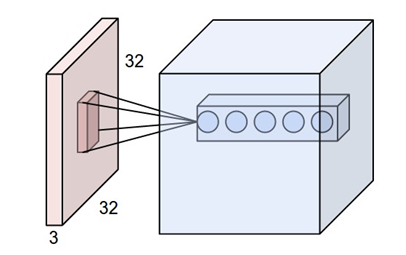
\includegraphics[width=0.6\textwidth]{./imgs/konvolucijski_sloj.png}
		\caption{Primjer ulazne slike 32x32x3 i rezultata izlaza nakon jednog konvolucijskog sloja dubine 5 \cite{CS231n}}
		\label{fg:konvolucijski_sloj}
	\end{center}
\end{figure}

Intuitivno konvolucijski slojevi će naučiti filtere koji će reagirati na određeni tip vizualnih svojstava, pa ima smisla dijeliti parametre filtera unutar svakog kanala neovisno o trenutno promatranom području slike.

Svaki filter ima onoliko pomičnih prozora koliko prethodni sloj ima kanala, a svaki pomični prozor ima prethodno određenu površinu receptivnog polja, npr. 3 prozora površine 3x3 kao u gornjem primjeru koji se pomiču po svom zaduženom kanalu. Moguće je svakom konvolucijskom filteru definirati korak (engl. stride) kojim se prozor pomiče po kanalima prethodnog sloja. Jedan položaj filtera daje jednu vrijednost u jednom izlaznom kanalu. Izlaz filtera je suma svih izlaza pojedinačnih prozora po kanalu (Slika \ref{fg:konvolucija}). Svaki prozor sa slike množi određenom težinom element na odgovarajućem mjestu te sumira dobivene vrijednosti svih prozora dobivajući vrijednost krajnjeg izlaza. Nakon izračuna svih vrijednosti sloja one se šalju u aktivacijsku funkciju i koriste se kao ulaz u sljedeće slojeve. 

\begin{figure}[!ht]
	\begin{center}
		\captionsetup{justification=centering}
		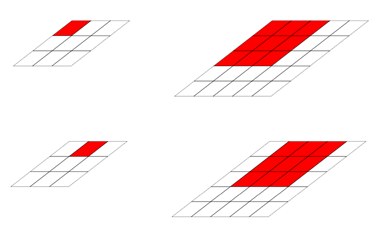
\includegraphics[width=0.6\textwidth]{./imgs/konvolucija.png}
		\caption{Primjer računanja izlaza (Lijevo) iz ulaza koji sadrži jedan kanal (Desno) pomicanjem prozora po kanalu \cite{DubokoUcenje}}
		\label{fg:konvolucija}
	\end{center}
\end{figure}

Korak pomaka (engl. stride) definira za koliko elemenata će se pomicati filter, odnosno svaki prozor, pri računanju izlazne vrijednosti sljedećeg neurona. Veći korak utječe na dimenziju izlaznog sloja (Slika \ref{fg:pomak}).

\begin{figure}[!ht]
	\begin{center}
		\captionsetup{justification=centering}
		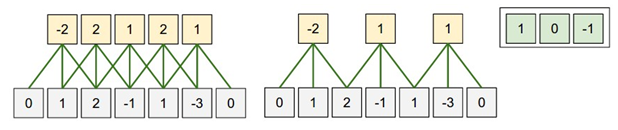
\includegraphics[width=0.6\textwidth]{./imgs/pomak.png}
		\caption{Utjecaj iznosa pomaka filtera na izlaze s prikazanim težinama na desnoj strani slike \cite{CS231n}}
		\label{fg:pomak}
	\end{center}
\end{figure}

Osim koraka pomaka, na dimenziju izlaza utječe i površina receptivnog polja filtera. Veće receptivno polje uzrokovat će manji broj izlaza jer će se na ulaznu sliku moći posložiti manja količina prozora iz kojih se računaju izlazne vrijednosti. Uobičajena praksa je proširiti ulaznu sliku dodavanjem nula (engl. padding) na rubove kako bi se nakon konvolucije zadržala dimenzija izlaza jednaka ulazu. Količina nula koje je potrebno dodati ovisi o receptivnom polju i koraku konvolucije.

Dodavanjem slojeva receptivno polje novih neurona se povećava ovisno o receptivnom polju prošlih neurona. Primjerice, nakon dvije konvolucije s receptivnim poljem 3x3 i korakom jedan, neuroni u drugom sloju vide veću površinu originalne slike od neurona u sloju prije njih (Slika \ref{fg:receptivno_polje}). Zbog toga se dublji slojevi konvolucijske mreže uče prepoznavati složenije vizualne značajke poput kotača, dok niži slojevi uče prepoznavati jednostavne značajke poput rubova objekata. 

\begin{figure}[!ht]
	\begin{center}
		\captionsetup{justification=centering}
		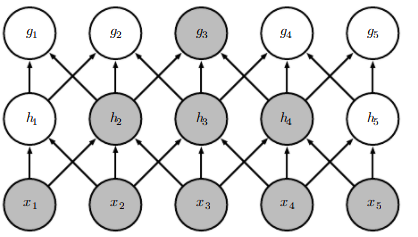
\includegraphics[width=0.6\textwidth]{./imgs/receptivno_polje.png}
		\caption{Povećanje receptivnog polja s dubinom mreže  \cite{deeplearningbook}}
		\label{fg:receptivno_polje}
	\end{center}
\end{figure}

\subsection{Slojevi sažimanja}

Sloj sažimanja je vrlo jednostavan, ali i vrlo bitan dio konvolucijske mreže. Sažimanje obično računa neku statističku vrijednost nad receptivnim poljem poput maksimalne vrijednosti ili srednje vrijednosti. Svrha sloja sažimanja je smanjiti dimenzionalnost (Slika \ref{fg:sazimanje}) i broj potrebnih parametara mreže. Dodatni pozitivan efekt smanjena broja parametara je i smanjenje vjerojatnosti da se takva mreža prenauči na ulazne podatke.

Osim reduciranja dimenzionalnosti, slojevi sažimanja unose invarijantnost na pomake u slici. Do intuitivnog objašnjenja prethodne tvrdnje možemo doći ako pretpostavimo da filter reagira na neki oblik u prethodnom sloju što prepoznajemo po većoj pozitivnoj vrijednosti izlaza od ostalih susjednih neurona (Slika \ref{fg:sazimanje}). Budući da za klasifikaciju nije bitno znati gdje se oblik nalazi na slici nego nalazi li se na slici, može se iskoristiti sažimanje maksimalnom vrijednošću. Takvo sažimanje će u sljedeće slojeve propustiti samo maksimalni odziv u promatranom prozoru (Slika \ref{fg:sazimanje2}).

\begin{figure}[H]
	\begin{center}
		\captionsetup{justification=centering}
		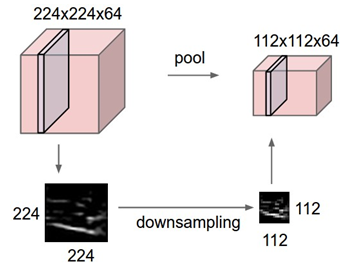
\includegraphics[width=0.6\textwidth]{./imgs/sazimanje.png}
		\caption{Sloj sažimanja s receptivnim poljem veličine 2x2 i pomakom 2 \cite{CS231n}}
		\label{fg:sazimanje}
	\end{center}
\end{figure}


\begin{figure}[H]
	\begin{center}
		\captionsetup{justification=centering}
		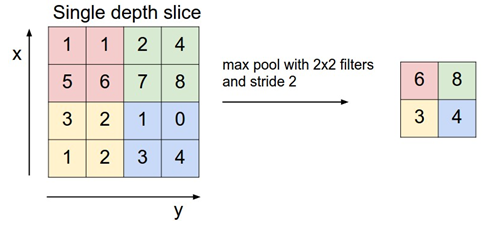
\includegraphics[width=0.6\textwidth]{./imgs/sazimanje2.png}
		\caption{Primjer sažimanja maksimalnom vrijednošću filterom 2x2 i pomakom 2 \cite{CS231n}}
		\label{fg:sazimanje2}
	\end{center}
\end{figure}

\subsection{Potpuno povezani slojevi}

Potpuno povezani slojevi dolaze iz najjednostavnijeg oblika neuronskih mreža, potpuno povezanih unaprijednih mreža, zbog čega će ovi slojevi biti objašnjeni izravno objašnjavanjem načina rada te vrste arhitekture mreža.
 
Potpuno povezana unaprijedna neuronska mreža je građena od slojeva koji se razlikuju jedino po aktivacijskoj funkciji: ulazni sloj na koji stižu podaci čija je aktivacija funkcija identiteta, skrivenih slojeva na čijem se izlazu nalazi neka derivabilna nelinearna funkcija te izlaznog sloja s konačnim rezultatom izračuna s aktivacijom prikladnom za problem koji se nastoji riješiti (Slika \ref{fg:potpuno_povezana}). Svaki ulaz u neuron ima svoju težinu koja množi ulaz te se svi ulazi na kraju sumiraju i šalju u aktivacijsku funkciju. Rezultat aktivacijske funkcije zatim postaje ulaz u sljedeće slojeve ili predstavlja završni rezultat iz zadnjeg sloja.

\begin{figure}[!ht]
	\begin{center}
		\captionsetup{justification=centering}
		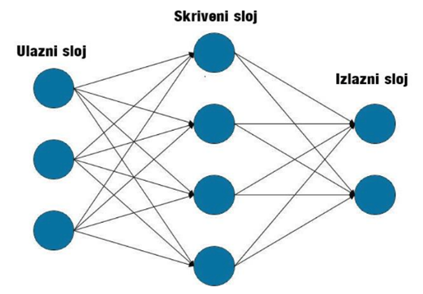
\includegraphics[width=0.6\textwidth]{./imgs/potpuno_povezana.png}
		\caption{Potpuno povezana unaprijedna neuronska mreža}
		\label{fg:potpuno_povezana}
	\end{center}
\end{figure}

\section{Analiza glavnih komponenti}

Analiza glavnih komponenti (engl. \textit{Principal component analysis - PCA}) standardni je alat u modernoj analizi podataka - u različitim područjima od neuroznanosti do računalne grafike zbog toga što je jednostavna, neparametarska metoda za ekstrahiranje relevantnih informacija iz podatkovnog skupa \cite{PCA}.

Bez ulaženja u matematiku koja se može pronaći u radu \cite{PCA}, \textit{PCA} se može objasniti laičkim terminima kao tehnika koja pronalazi temeljne varijable koje najbolje diferenciraju podatkovni skup (poznatije kao glavne komponente - engl. principal components). Glavne komponente skupa su dimenzije po kojima je naš podatkovni skup najviše raspršen (Slika \ref{fg:pca_start}).

\begin{figure}[!ht]
	\begin{center}
		\captionsetup{justification=centering}
		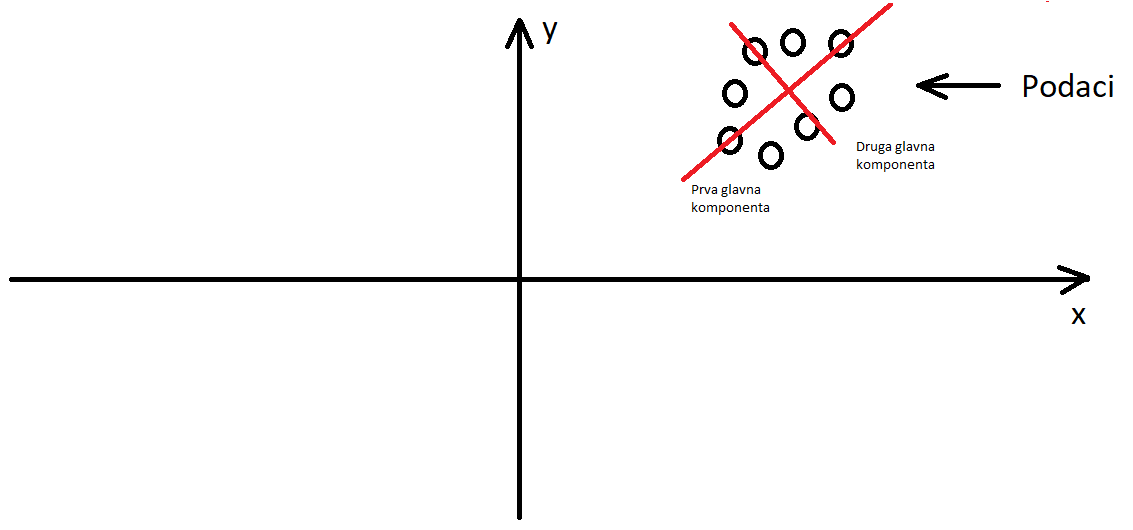
\includegraphics[width=0.6\textwidth]{./imgs/pca_start.png}
		\caption{Određivanje glavnih komponenti podatkovnog skupa}
		\label{fg:pca_start}
	\end{center}
\end{figure}

Nakon što je određen traženi broj glavnih komponenti, u slučaju sa slike njih dva, podatkovni skup se transformira u novi koordinatni sustav (Slika \ref{fg:pca_end}) čije su koordinatne osi dekorelirane.

\begin{figure}[H]
	\begin{center}
		\captionsetup{justification=centering}
		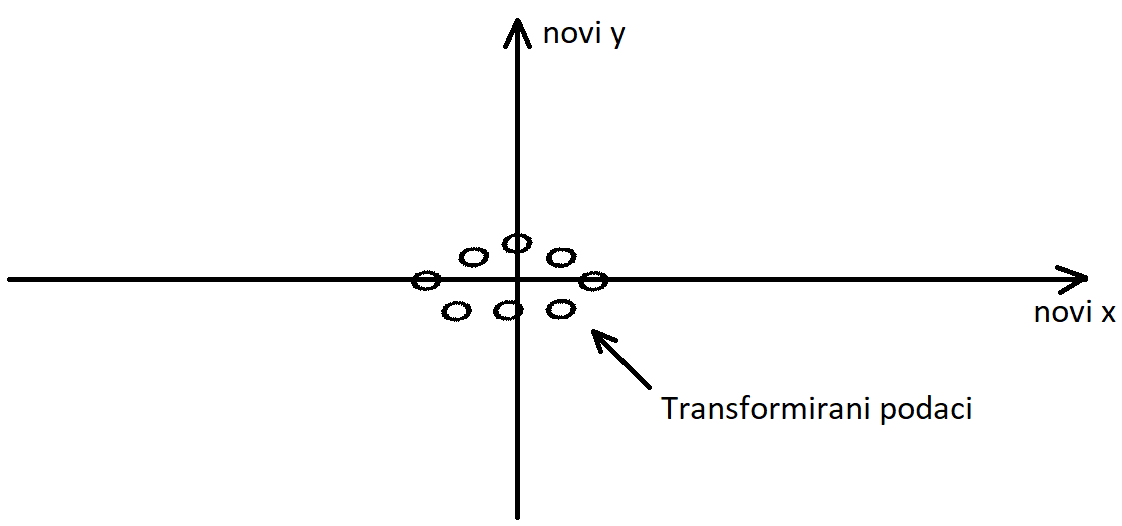
\includegraphics[width=0.6\textwidth]{./imgs/pca_end.png}
		\caption{Transformirani podatkovni skup}
		\label{fg:pca_end}
	\end{center}
\end{figure}

Iako se u gore navedenom primjeru dimenzionalnost podataka ne reducira (2D podaci ostaju u 2D prostoru), već se oni samo dekoreliraju, glavno područje primjene \textit{PCA} tehnike je upravo redukcija dimenzionalnosti koja funkcionira na skoro identičan način. Upotreba \textit{PCA} metode za redukciju dimenzionalnosti razlikuje se po tome što se nakon određenih smjerova raspršenja oni poredaju silazno po svojstvenim vrijednostima te se odabere željena dimenzija na koju se podaci žele transformirati. Nakon što se završi transformacija na manji broj dimenzija ostale glavne komponente s nižim svojstvenim vrijednostima se gube. 

Važno je naglasiti da je glavna motivacija iza \textit{PCA} tehnike uklanjanje korelacije u podatkovnom skupu, odnosno uklanjanje zavisnosti drugog reda između podataka [3]. Način na koji \textit{PCA} nastoji ostvariti taj cilj je pretpostavkom da su glavne komponente međusobno ortogonalne zbog čega \textit{PCA} neće biti primjerena za podatkovne skupove poput onog na slici \ref{fg:pca_problem}.

\begin{figure}[H]
	\begin{center}
		\captionsetup{justification=centering}
		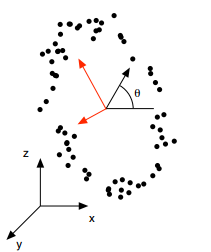
\includegraphics[width=0.4\textwidth]{./imgs/pca_problem.png}
		\caption{Podatkovni skup i crveno odabrane glavne komponente \cite{PCA}}
		\label{fg:pca_problem}
	\end{center}
\end{figure}


\section{VGG}

Arhitektura prvog isprobanog modela datira iz 2014. godine, a dolazi sa sveučilišta Oxford čiji ju je tim koristio u \textit{ImageNet} natjecanju.\textit{VGG} tim (engl. \textit{Visual Geometry Group}), po kojem je mreža dobila ime, ostvario je prvo mjesto iz zadatka lokalizacije objekata i drugo mjesto iz zadatka klasifikacije.

Njihov glavni doprinos je temeljita evaluacija arhitektura dubokih mreža koje koriste konvolucijske filtere malih dimenzija (3x3), čime su pokazali da se značajno poboljšanje u odnosu na tadašnje najbolje arhitekture može postići povećanjem dubine mreže na 16-19 slojeva dubine \cite{VGG}. 

Nakon evaluiranja više konfiguracija mreža, \textit{VGG} tim je pokazao da dublja konvolucijska mreža nadmašuje rezultate mreža s manje slojeva, zbog čega smo u našim ispitivanjima koristili njihovu najdublju mrežu u stupcu E sa slike \ref{fg:vgg}.

\begin{figure}[!ht]
	\begin{center}
		\captionsetup{justification=centering}
		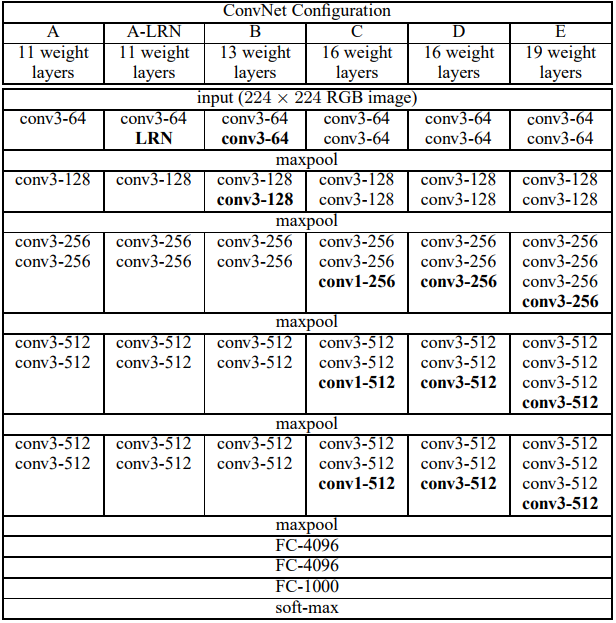
\includegraphics[width=0.6\textwidth]{./imgs/vgg.png}
		\caption{Konfiguracije VGG tima \cite{VGG}. Parametri konvolucije su prikazani kao conv<dimenzije filtera>-<broj kanala>, a nakon svake se nalazi ReLU aktivacija koja nije prikazana}
		\label{fg:vgg}
	\end{center}
\end{figure}

\section{Inception v4}

\textit{Inception v4} model je Google-ova četvrta iteracija \textit{Inception} arhitekture koja se od \textit{VGG} arhitekture najviše razlikuje po svojoj “širini”.  Arhitektura mreže u skraćenom prikazu \textit{Inception} blokova se može vidjeti na slici (Slika \ref{fg:inceptionv4}). 

\begin{figure}[!ht]
	\begin{center}
		\captionsetup{justification=centering}
		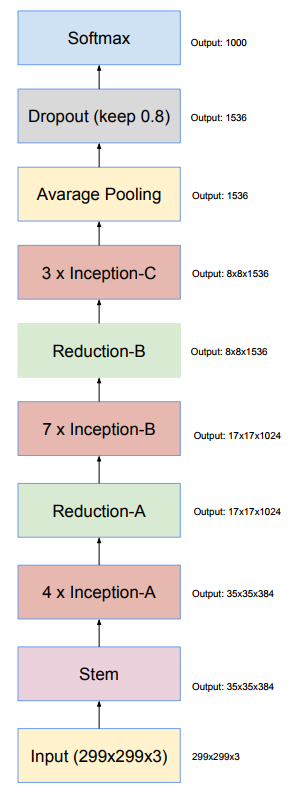
\includegraphics[width=0.4\textwidth]{./imgs/inceptionv4.png}
		\caption{Inception v4 \cite{Inceptionv4}}
		\label{fg:inceptionv4}
	\end{center}
\end{figure}

\textit{Inception} blokovi su postali popularni nakon što je Google-ova tadašnja arhitektura \textit{GoogLeNet} izgrađena od \textit{Inception} blokova ostvarila dobre performanse na natjecanju ImageNet. Njihova glavna prednost je rješavanje problema odabira dimenzija filtera pri izgradnji mreže jer se sastoje od više grana konvolucija koje ulazni podatak obrađuju s različitim dimenzijama filtera. Zbog stablaste razgranatosti, \textit{Inception} blok iz ulaza može prepoznati kompliciranije uzorke jer svaka grana ulazni podatak promatra s različitim receptivnim poljem (Slika \ref{fg:inception_blok_a}).
	
\begin{figure}[H]
	\begin{center}
		\captionsetup{justification=centering}
		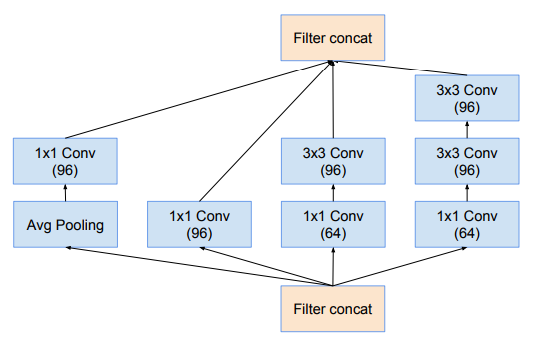
\includegraphics[width=0.6\textwidth]{./imgs/inception_blok_a.png}
		\caption{Inception-A blok  \cite{Inceptionv4}}
		\label{fg:inception_blok_a}
	\end{center}
\end{figure}

\textit{Inception} moduli, od kojih je građena mreža (A-C), obrađuju ulaze na sličan način. Zajednička karakteristika im je da izlazne dimenzije podatka ostaju jednake (npr. \textit{Inception-A} na ulazu prima 35x35x384 a na izlazu daje 35x35x384), a razlikuju se po načinu obrade ulaznog podatka, točnije broja konvolucijskih slojeva u granama i njihovih parametara.

Osim \textit{Inception} modula, mreža se sastoji i od \textit{Reduction} blokova koji su, uz ekstrakciju značajki, zaslužni za smanjivanje dimenzionalnosti ulaznog podatka. Kao i \textit{Inception} blokovi razlika između \textit{Reduction-A} bloka i \textit{Reduction-B} bloka je samo u parametrima grana i dizajnu grana, a oba bloka smanjuju širinu i visinu ulaznog podatka za faktor 2 korištenjem slojeva sažimanja ili konvolucija s korakom 2 (Slika \ref{fg:inception_reduction_a}).

\begin{figure}[!ht]
	\begin{center}
		\captionsetup{justification=centering}
		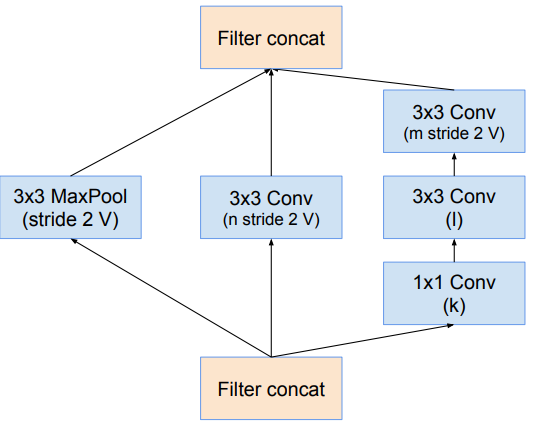
\includegraphics[width=0.6\textwidth]{./imgs/inception_reduction_a.png}
		\caption{Reduction-A blok (za Inception v4 k=192, l=224, m=256, n=384) \cite{Inceptionv4}}
		\label{fg:inception_reduction_a}
	\end{center}
\end{figure}
%%%%%%%%%%%%%%%%%%%%%%%%%%%%%%%%%%%%%%%%%%%%%%%%%%%%%%%%%%%%%%%%%%%%%%%%%%%%%%%%%%%%%%%
%% CHAPTER
\chapter{Rezultati i rasprava}

\section{Metrike sličnosti}

Prilikom uspoređivanja sličnosti vektora isprobali smo dvije metrike, euklidsku i kosinusnu udaljenost. 

Euklidska udaljenost definirana je kao L2 udaljenost između dva vektora (\ref{eq:euklidska_udaljenost}), a raspon vrijednosti iznosi od nula, za točke koje se nalaze na istom mjestu u prostoru, do beskonačnosti. Negativna strana euklidske udaljenosti je zanemarivanje informacija o kutu između dvije točke. Primjer te situacije se može vidjeti na slici \ref{fg:euklidska_udaljenost} gdje su točka P, Q i R jednako udaljene od točke M, no kada bismo uzimali informaciju o kutu u obzir najsličnija bi nam bila točka P \cite{VectorSimilarity}.

\begin{equation}
\label{eq:euklidska_udaljenost}
EuclideanDistance(x,y) = \sqrt{\sum_{i=1}^n (x_i-y_i)^2}    
\end{equation}

\begin{figure}[!ht]
	\begin{center}
		\captionsetup{justification=centering}
		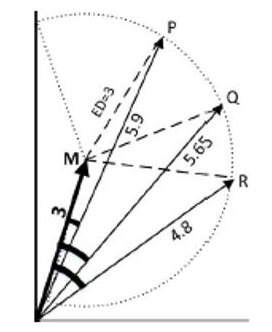
\includegraphics[width=0.3\textwidth]{./imgs/euklidska_udaljenost.png}
		\caption{Primjer euklidske udaljenosti \cite{VectorSimilarity}}
		\label{fg:euklidska_udaljenost}
	\end{center}
\end{figure}

Kosinusna udaljenost je definirana kao jedan minus skalarni produkt dva vektora podijeljen s umnoškom njihovih normi (\ref{eq:kosinusna_udaljenost}), a raspon vrijednosti je od 2, za vektore koji gledaju u suprotnim smjerovima, do 0, za kolinearne vektore. Negativna strana kosinusne udaljenosti je zanemarivanje duljine vektora. Primjer se može vidjeti na \ref{fg:kosinusna_udaljenost} gdje su točke B, C i D jednako udaljene od točke A jer zatvaraju jednak kut, no kada bi se promatrala njihova euklidska udaljenost dobili bismo različite rezultate \cite{VectorSimilarity}.

\begin{equation}
\label{eq:kosinusna_udaljenost}
CosineDistance(x,y) = 1- cos(\pmb x, \pmb y) = 1 - \frac {\pmb x \cdot \pmb y}{||\pmb x|| \cdot ||\pmb y||}
\end{equation}

\begin{figure}[!ht]
	\begin{center}
		\captionsetup{justification=centering}
		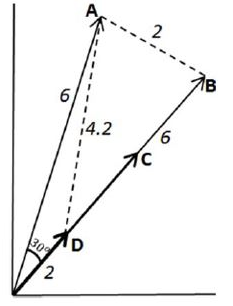
\includegraphics[width=0.3\textwidth]{./imgs/kosinusna_udaljenost.png}
		\caption{Primjer kosinusne udaljenosti \cite{VectorSimilarity}}
		\label{fg:kosinusna_udaljenost}
	\end{center}
\end{figure}

Obje metrike su davale skoro identične rezultate uz male promjene poretka između vraćenih slika. Jedan od razloga zašto smo dobili takve rezultate je velika dimenzionalnost prostora kojeg vektori razapinju. Posljedica toga je da dvije točke koje se nalaze blizu u prostoru ujedno zatvaraju i maleni kut zbog čega se smatraju sličnima u obje metrike.	

Nakon ispitivanja rezultata metrika, odabrali smo kosinusnu udaljenost koja je davala zadovoljavajuće rezultate. Potencijalni problemi koji se mogu pojaviti kod te metrike u našem slučaju nisu pretjerano bitni budući da nam nije bitna duljina vektora već njegovo usmjerenje, odnosno relativan iznos aktivacija koje taj vektor opisuje. Primjerice, ako našem sustavu predamo sliku mačke i tražimo ostale slične slike, želimo vratiti sve vektore kojima su dominantni elementi koji detektiraju oči, njušku, uši mačke. Zbog toga nam je kosinusna udaljenost zadovoljavajuća jer vraća slike čiji reprezentativni vektori imaju jednak odnos dominantnih elemenata unutar vektora.


\section{Predtrenirana arhitektura VGG}

\textit{VGG} arhitektura je prva isprobana mreža za ekstrakciju značajki, točnije njezin posljednji sloj konvolucijskog dijela mreže. Težinski koeficijenti mreže preuzeti su iz pobjedničke arhitekture ImageNet natjecanja čiji su filteri već naučeni prepoznavati komplicirane uzorke na ulaznim slikama.

Ulazna slika u mrežu je dimenzija 224x224x3, a finalni rezultat sloja kojeg koristimo je vektor od 25.000 elemenata. Budući da je krajnji cilj ostvariti reprezentaciju slike vektorom manjih dimenzija, što bi omogućilo brže pretraživanje, rezultat konvolucijske mreže se \textit{PCA} modelom dalje reducira na 3000 dimenzija. Za treniranje \textit{PCA} modela nasumično je izabrano 50.000 slika kako bismo dobili što bolju procjenu glavnih komponenti.

Rezultati dobiveni na ovaj način za pojedine slike daju očekivane rezultate  (Slika \ref{fg:auti_vgg}), dok za druge već u top 5 najsličnijih slika vidimo nepovezanost rezultata (Slika \ref{fg:greske_vgg}). 

\begin{figure}[!ht]
	\begin{center}
		\captionsetup{justification=centering}
		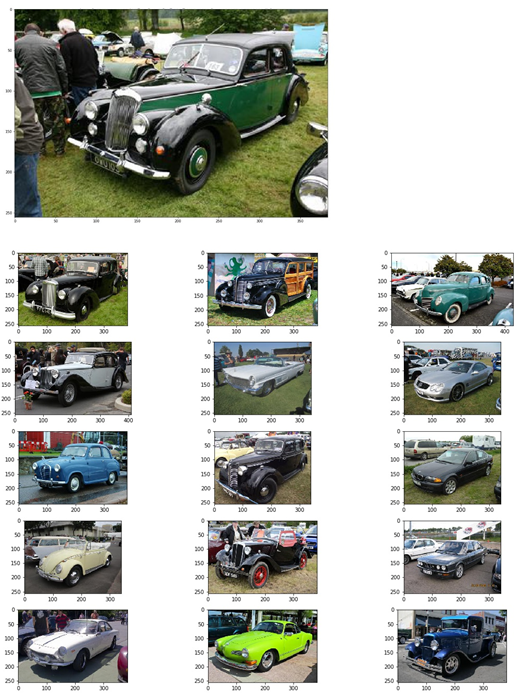
\includegraphics[width=0.8\textwidth]{./imgs/auti_vgg.png}
		\caption{Top 12 sličnih rezultata za sliku na vrhu}
		\label{fg:auti_vgg}
	\end{center}
\end{figure}

\begin{figure}[H]
\begin{center}
	\captionsetup{justification=centering}
	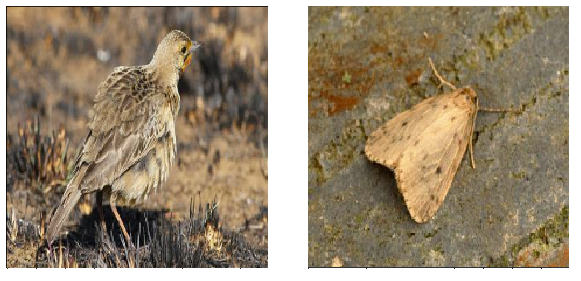
\includegraphics[width=0.8\textwidth]{./imgs/greske_vgg.png}
	\caption{Slika na temelju koje se rade preporuka (lijevo) i slika u top 5 koja nije ispravna (desno)}
	\label{fg:greske_vgg}
\end{center}
\end{figure}

Dobri rezultati sažimanja, kao i lažni pozitivi dobiveni korištenjem jednostavnog \textit{VGG} modela, u daljnjim testiranjima koristili smo kao referencu uspješnosti ekstrakcije značajki iz ulazne slike kod kompliciranijih modela.

\section{Predtrenirana arhitektura Inceptionv4}

Sljedeća arhitektura sa značajno većim kapacitetom je \textit{Inception v4}. Kao i u slučaju arhitekture \textit{VGG} i za \textit{Inception v4} smo preuzeli težinske koeficijente iz arhitekture naučene na skupu ImageNet.

Vođeni zaključcima koje smo dobili testirajući arhitekturu \textit{VGG} za dohvaćanje sličnih slika, prvi način ekstrakcije značajki, kao i u arhitekturi \textit{VGG}, bio je uzimanje izlaza zadnjeg sloja konvolucijske mreže. U ovom slučaju to je vektor od 1536 elemenata dobiven globalnim sažimanjem prosječnom vrijednošću. Dobiveni vektori su se kasnije, korištenjem \textit{PCA} modela, reducirali na 300 elemenata što je dalo loše rezultate unatoč velikom kapacitetu mreže (Slika \ref{fg:inception_zadnji_sloj_auti_greska}).

\begin{figure}[H]
	\begin{center}
		\captionsetup{justification=centering}
		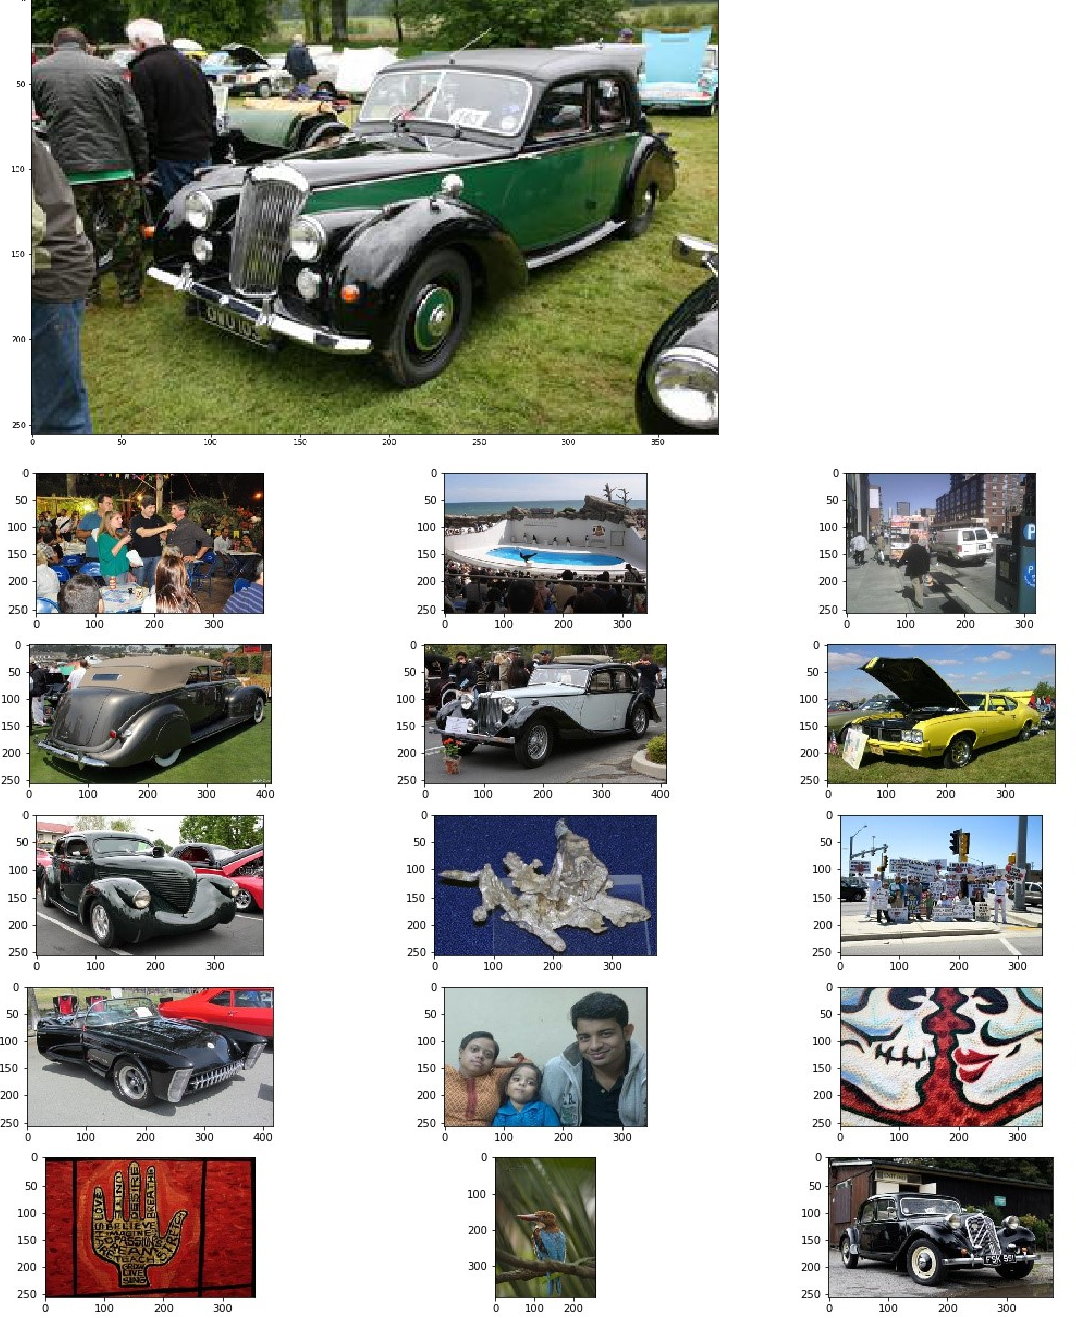
\includegraphics[width=0.8\textwidth]{./imgs/inception_zadnji_sloj_auti_greska.png}
		\caption{Top 12 sličnih rezultata za sliku na vrhu}
		\label{fg:inception_zadnji_sloj_auti_greska}
	\end{center}
\end{figure}

Razlog zašto redukcija predzadnjeg sloja dovodi do ovoliko loših rezultata djelomično se može objasniti time što mreža taj sloj koristi za završnu klasifikaciju i time nema neku semantičku interpretaciju. Budući da je krajnji cilj dobiti vektor koji se sastoji od 300 elemenata gdje je intenzitet svakog elementa u vektoru označava pojavljivanje određenog uzorka na ulaznoj slici, odlučili smo značajke ekstrahirati kao maksimalni odziv svakog konvolucijskog sloja. 

Ekstrakcija značajki se vrši se na način da se nad svakim konvolucijskim slojem u \textit{Inception} mreži napravi operacija globalnog sažimanja. Na primjer, ako je izlaz konvolucijskog sloja 12 x 12 x 512 (visina, širina, broj kanala), globalnim sažimanjem svakog od kanala dobiti ćemo vektor 1x1x512. Dobiveni vektori svakog konvolucijskog sloja nakon globalnog sažimanja se izravnaju i konkateniraju u jedan veliki vektor s  \textasciitilde16000 elemenata.  Tako dobiveni elementi se zatim reduciraju na vektore od 300 elemenata korištenjem \textit{PCA} modela. Kako bi rezultati bili što precizniji, korišteni \textit{PCA} model je prethodno istreniran korištenjem 100.000 ekstrahiranih vektora nasumično odabranih slika radi preciznijeg određivanja glavnih komponenti podatkovnog skupa.

Primjer tako dobivenih rezultata može se vidjeti na sljedećim slikama \ref{fg:inception_globalno_sazimanje_auti}, \ref{fg:inception_globalno_sazimanje_ptice}, \ref{fg:inception_globalno_sazimanje_ptice}, a korišteni kod za generiranje kao i dodatne rezultate moguće je vidjeti na \cite{AVSP}.

\begin{figure}[H]
	\begin{center}
		\captionsetup{justification=centering}
		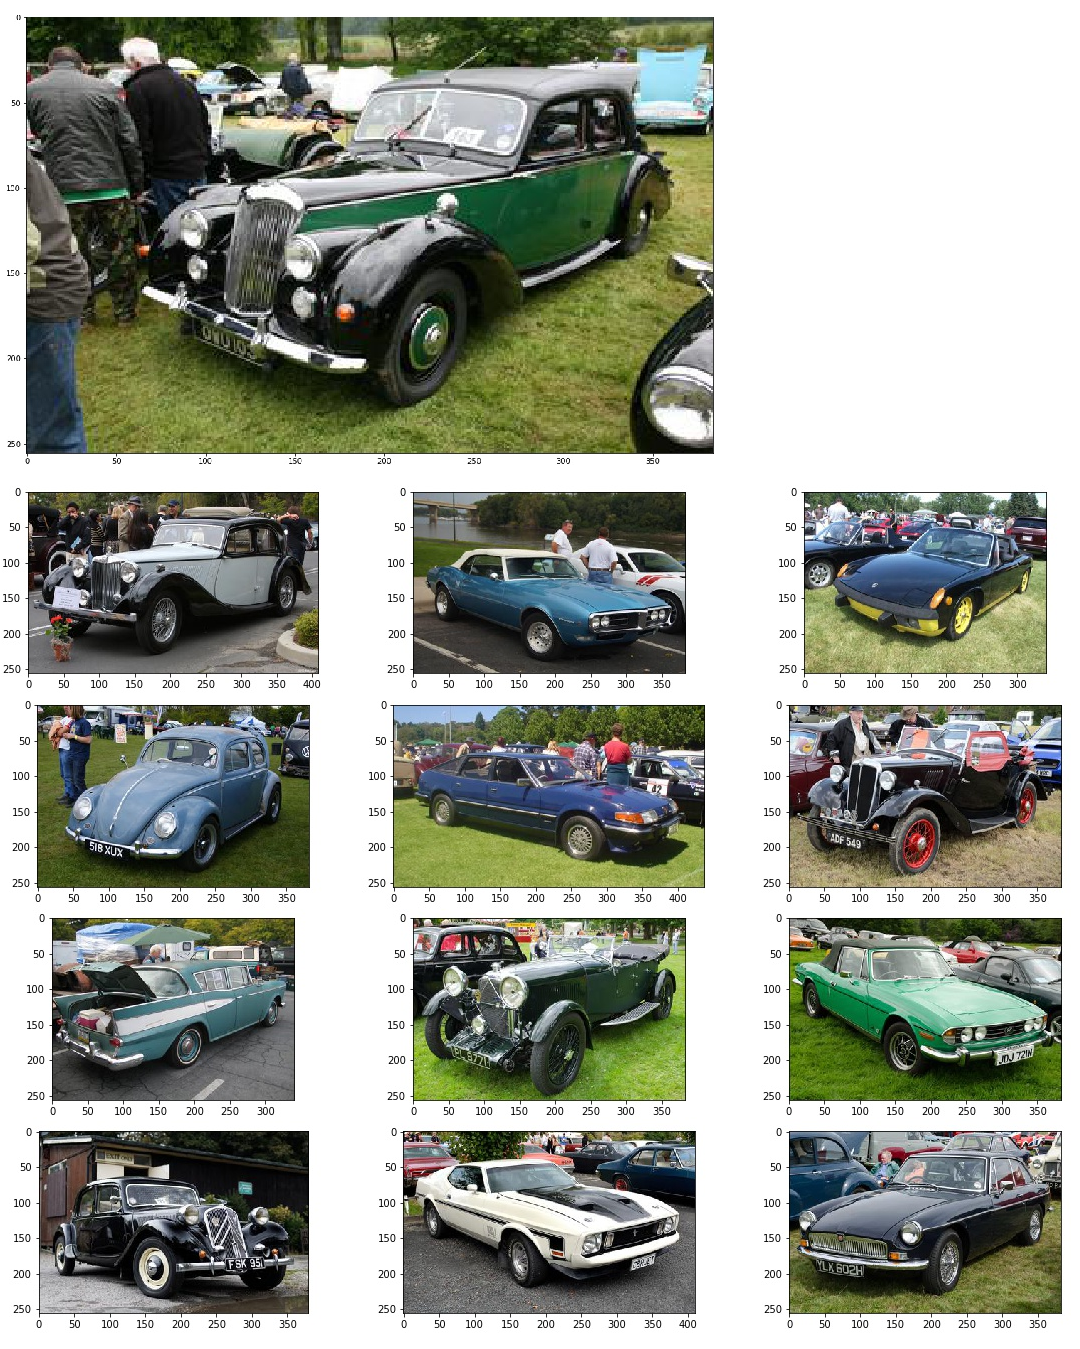
\includegraphics[width=0.8\textwidth]{./imgs/inception_globalno_sazimanje_auti.png}
		\caption{Top 12 sličnih rezultata za sliku na vrhu}
		\label{fg:inception_globalno_sazimanje_auti}
	\end{center}
\end{figure}

\begin{figure}[H]
	\begin{center}
		\captionsetup{justification=centering}
		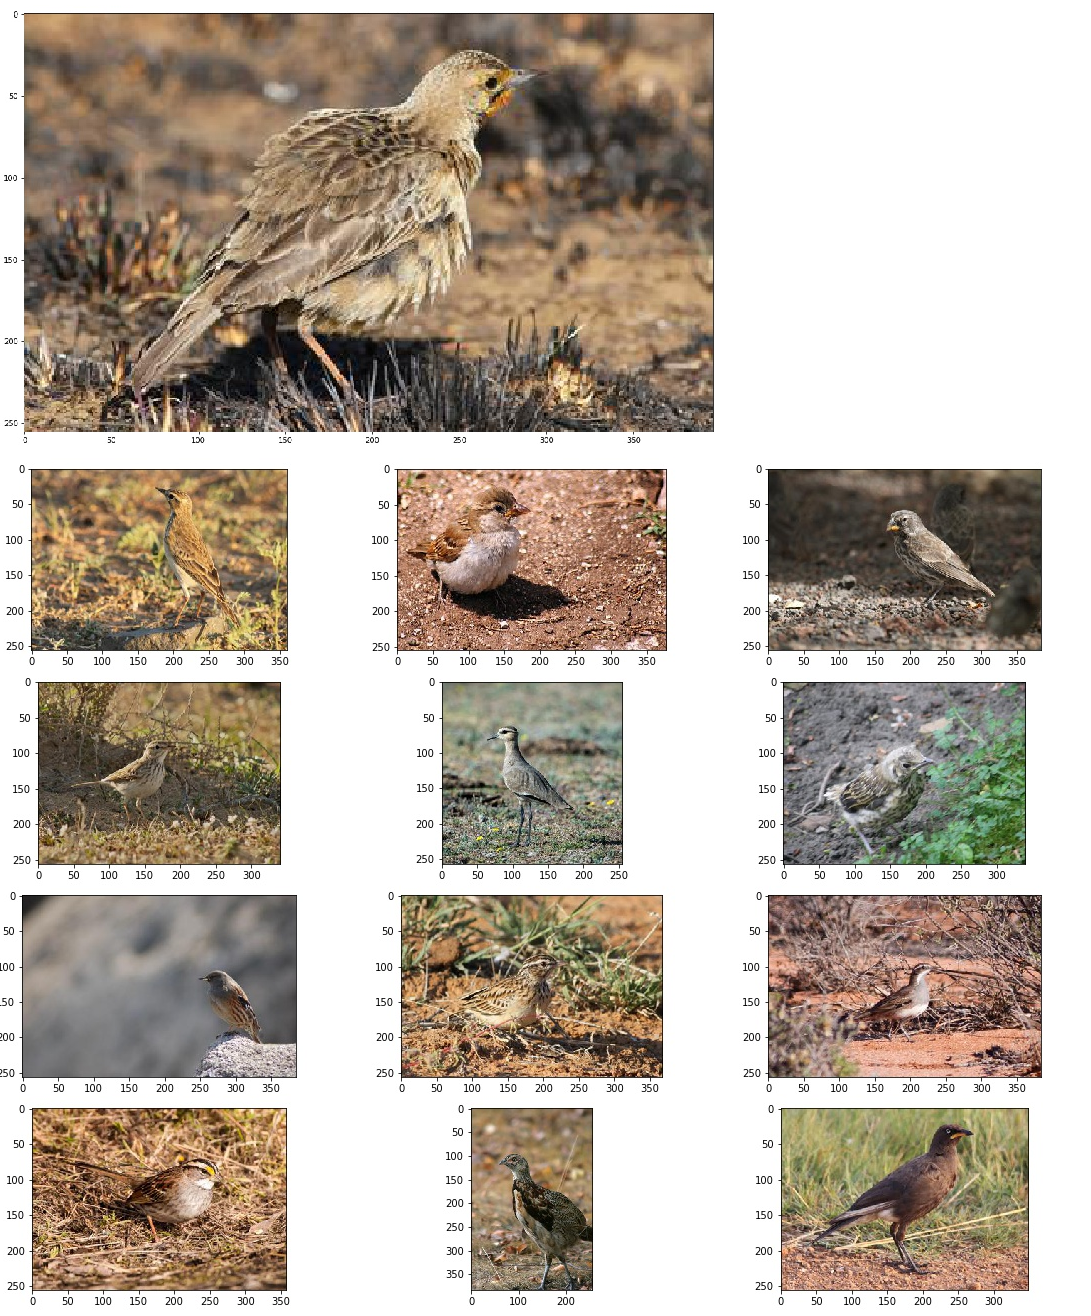
\includegraphics[width=0.8\textwidth]{./imgs/inception_globalno_sazimanje_ptice.png}
		\caption{Top 12 sličnih rezultata za sliku na vrhu}
		\label{fg:inception_globalno_sazimanje_ptice}
	\end{center}
\end{figure}


\begin{figure}[H]
	\begin{center}
		\captionsetup{justification=centering}
		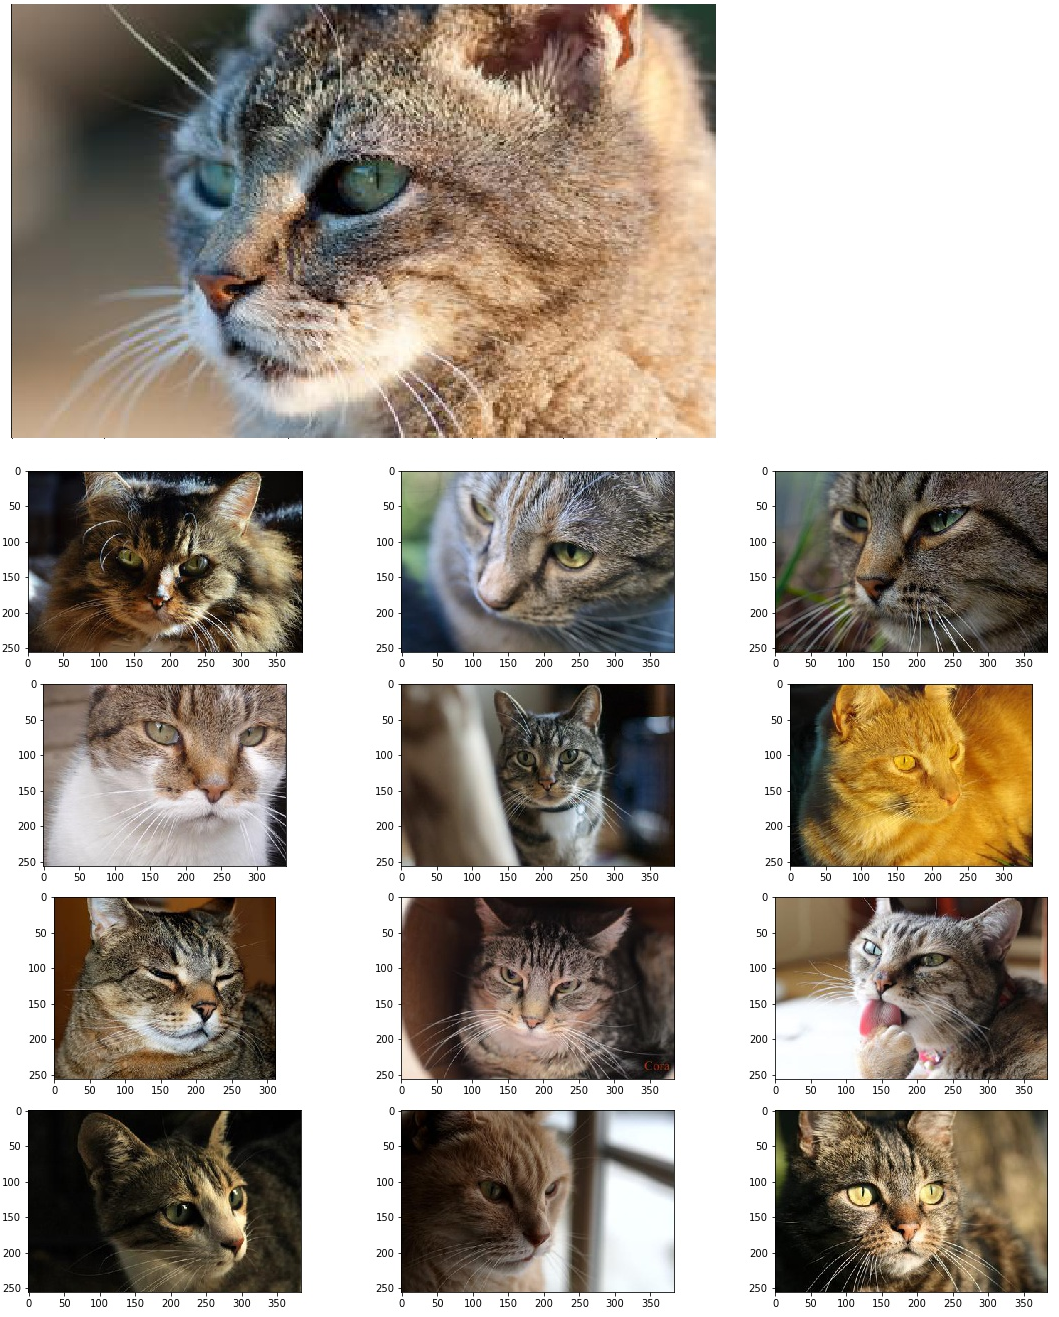
\includegraphics[width=0.8\textwidth]{./imgs/inception_globalno_sazimanje_macke.png}
		\caption{Top 12 sličnih rezultata za sliku na vrhu}
		\label{fg:inception_globalno_sazimanje_macke}
	\end{center}
\end{figure}

Kao što se vidi iz prikazanih slika moguće je reprezentirati sliku sa svega 300 elemenata što predstavlja višestruku uštedu prostora (\ref{tbl:usteda_prostora}) pri ćemu vektor i dalje dobro ekstrahira suštinu slike te slične grupira u bliske nakupine. To svojstvo je posebno vidljivo u sljedećem poglavlju.


\begin{table}[htb]
	\caption{Primjer uštede prostora}
	\label{tbl:usteda_prostora}
	\centering
	
	\begin{tabular}{lcc| c}
		\toprule
		{} & \thead{Dimenzije slike} & \thead{Ukupno elemenata} & \thead{Faktor uštede} \\
		\midrule
		\textit{{480p (12:9)}} & 640x480 & 921 600 & 307 200\%\\
		\textit{720p Widescreen} & 1280x720 &  2 764 800 & 921 600\%  \\		
		\textit{1080p HD Widescreen} & 1920x1080 &  6 220 800 & 2 073 600\%  \\
		
		\bottomrule
	\end{tabular}
\end{table}

\section{T-SNE prikaz smanjenog skupa podataka}

Budući da je korišteni podskup slika Google-ovog \textit{OpenImage} \cite{openimages} podatkovnog skupa velik (\textasciitilde1 milijun slika) i anotacije klasa nisu nužno točne jer ih je većina generirana automatskom strojnom anotacijom korištenjem servisa poput Google Cloud Vision API, za vizualizaciju smo odabrali manji skup podataka koji je anotiran ručno i precizno.

Odabrani skup podataka je \textit{STL-10} \cite{STL10} čije slike imaju dimenziju 96x96x3, a nastao je po uzoru na podatkovni skup CIFAR-10 koji se obično koristi za vrednovanje modela.

Ekstrahirane značajke, dobivene korištenjem najboljeg modela \textit{Inception v4} s globalnim sažimanjem kanala, su pomoću metode \textit{t-SNE} prikazane u 2D prostoru. Na slici \ref{fg:stl_10_tsne} se vidi da su podaci grupirani u nakupine uz poneka miješanja grupa poput slika jelena i konja. Razlog tome može biti vrlo slična pozadine slike i kut snimanja gdje se značajke jelena (rogovi) ne vide jasno na slici zbog čega ih mreža lako može zamijeniti zbog približno jednake boje i građe.

Moguće je dodatno poboljšati performanse predtrenirane mreže za određivanje sličnosti tako da se glavne komponente \textit{PCA} modela biraju samo na značajkama dobivenim iz klasa koje se žele preciznije razlikovati, u ovome slučaju klasa iz \textit{STL-10} podatkovnog skupa.

\begin{figure}[!ht]
	\begin{center}
		\captionsetup{justification=centering}
		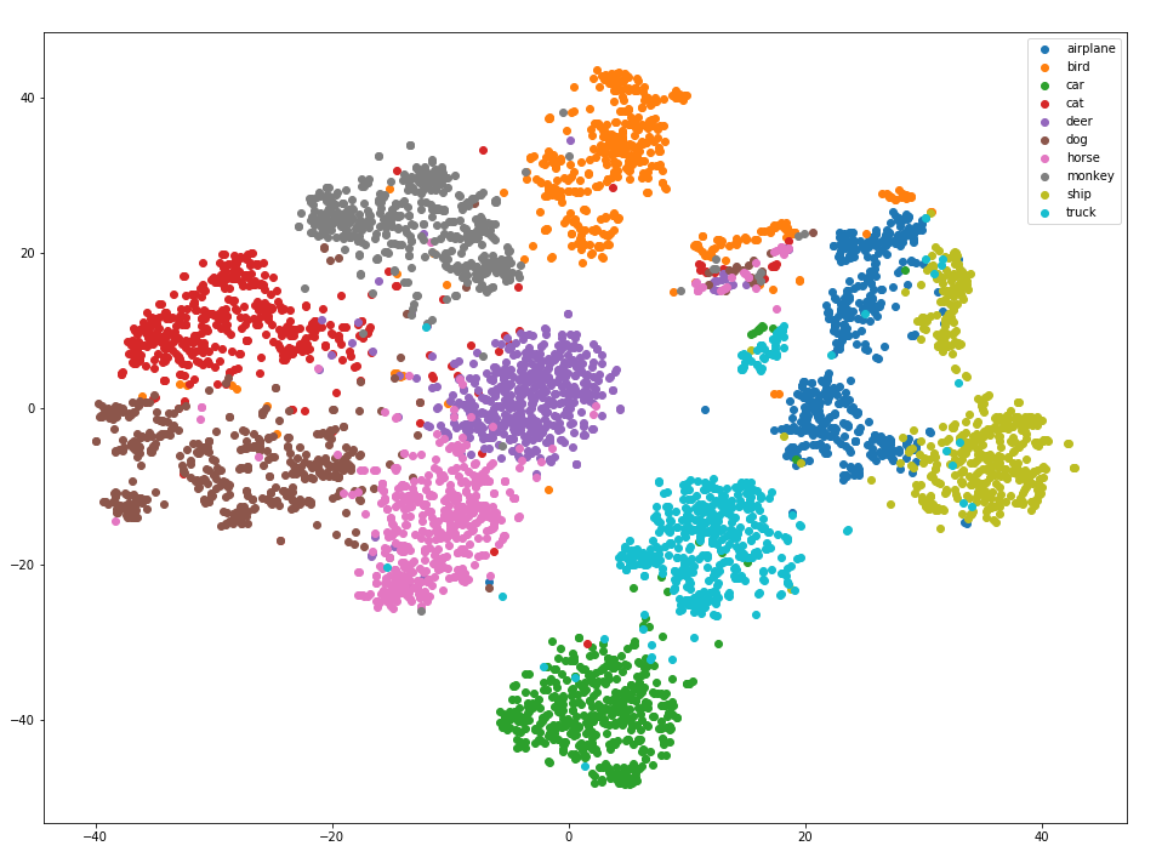
\includegraphics[width=1.\textwidth]{./imgs/stl_10_tsne.png}
		\caption{STL-10 dataset reprezentativni vektori prikazani u dvije dimenzije}
		\label{fg:stl_10_tsne}
	\end{center}
\end{figure}

%%%%%%%%%%%%%%%%%%%%%%%%%%%%%%%%%%%%%%%%%%%%%%%%%%%%%%%%%%%%%%%%%%%%%%%%%%%%%%%%%%%%%%%
%% CHAPTER
\chapter{Demo preporučitelj po sadržaju}

Kako bismo demonstrirali ponašanje razvijanog sustava za pronalaženje sličnih slika u sklopu projekta implementirana je i jednostavna \textit{web} aplikacija. 

Aplikacija je inspirirana sličnim proizvodom, društvenom mrežom temeljenom na dijeljenju slika pod nazivom Pinterest, koja organizira podatke poput slika i video zapisa s cijelog interneta \cite{wiki-pintrest}. 

Naš sustav karakterizira puno manji volumen podataka s kojim rukujemo, ali koncept ostaje isti: prepoznati preference korisnika na temelju njegovih interakcija sa sustavom i pronalazak relevantnih podataka kako bi se poboljšalo korisničko iskustvo.

Aplikacija omogućuje pregledavanje \textit{STL-10} skupa podataka gdje korisnik može izdvojiti skup slika od interesa na temelju kojih će sustav isfiltrirati sve slike sličnog konteksta.

Demo je implementiran kao \textit{web} aplikacija kako bismo sustav učinili što pristupačnijim novim korisnicima i postavljen je na \textit{Heroku} platformu \footnote{Izvršnoj verziji aplikacije moguće je pristupiti na linku \url{https://recommender-demo.herokuapp.com}.} .


\section{Tijek rada}

Ovaj odjeljak opisuje ponašanje sustava iz korisničke perspektive i kroz niz instrukcija daje pregled mogućnosti preporučitelja. Posjećivanjem navedene \textit{web} stranice aplikacije korisnik se usmjerava na obrazac za prijavu. Uz pretpostavku da korisnik nema profil za pristup stranici, potrebno je napraviti registraciju putem gumba 'Register' koji se nalazi u gornjem desnom kutu stranice. Pri dolasku na stranicu od korisnika se traži unos korisničkog imena, e-maila i lozinke te se po pritisku na 'Sign Up' gumb završava proces registracije (Slika \ref{fg:demo_register}). Ako su podaci ispravno uneseni, korisnik će biti vraćen na početnu stranicu gdje može iskoristiti kreirani račun za prijavu (Slika \ref{fg:demo_login}). 
 
\begin{figure}[!ht]
	\begin{center}
		\captionsetup{justification=centering}
		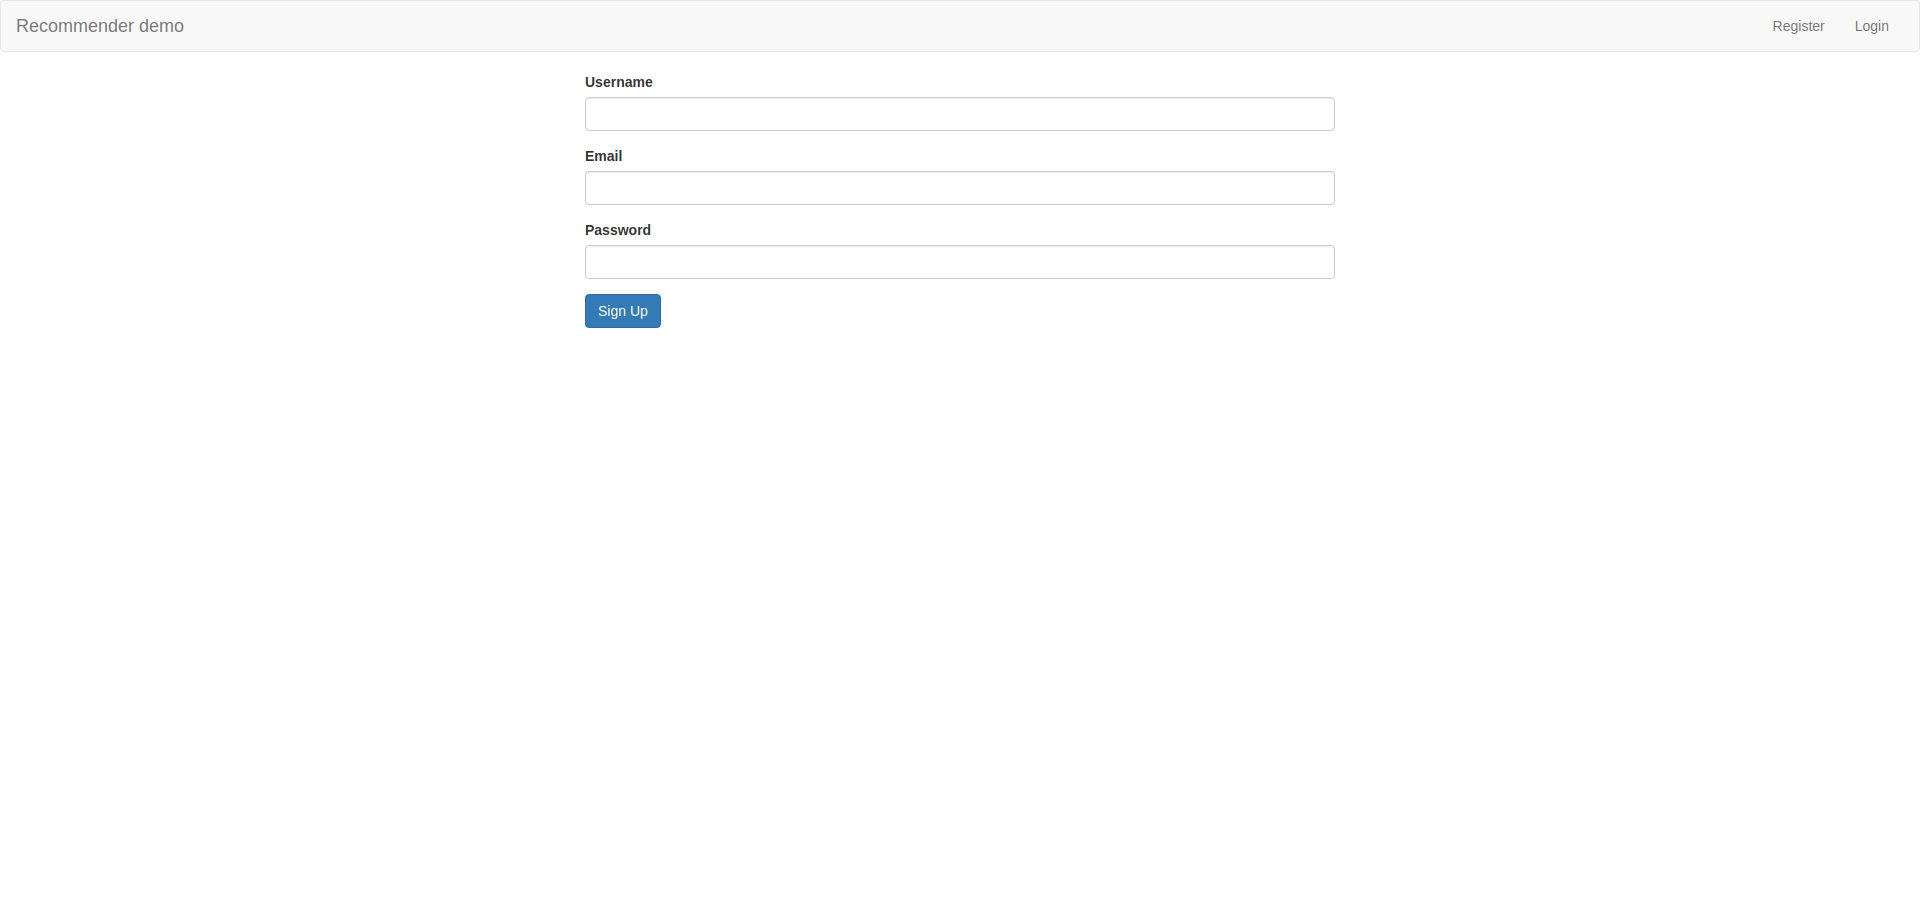
\includegraphics[width=1.0\textwidth]{./imgs/demo-preporucitelja-po-sadrzaju/tijek-rada/demo-regi.png}
		\caption{Stranica za registraciju novog korisnika}
		\label{fg:demo_register}
	\end{center}
\end{figure}

\begin{figure}[!ht]
	\begin{center}
		\captionsetup{justification=centering}
		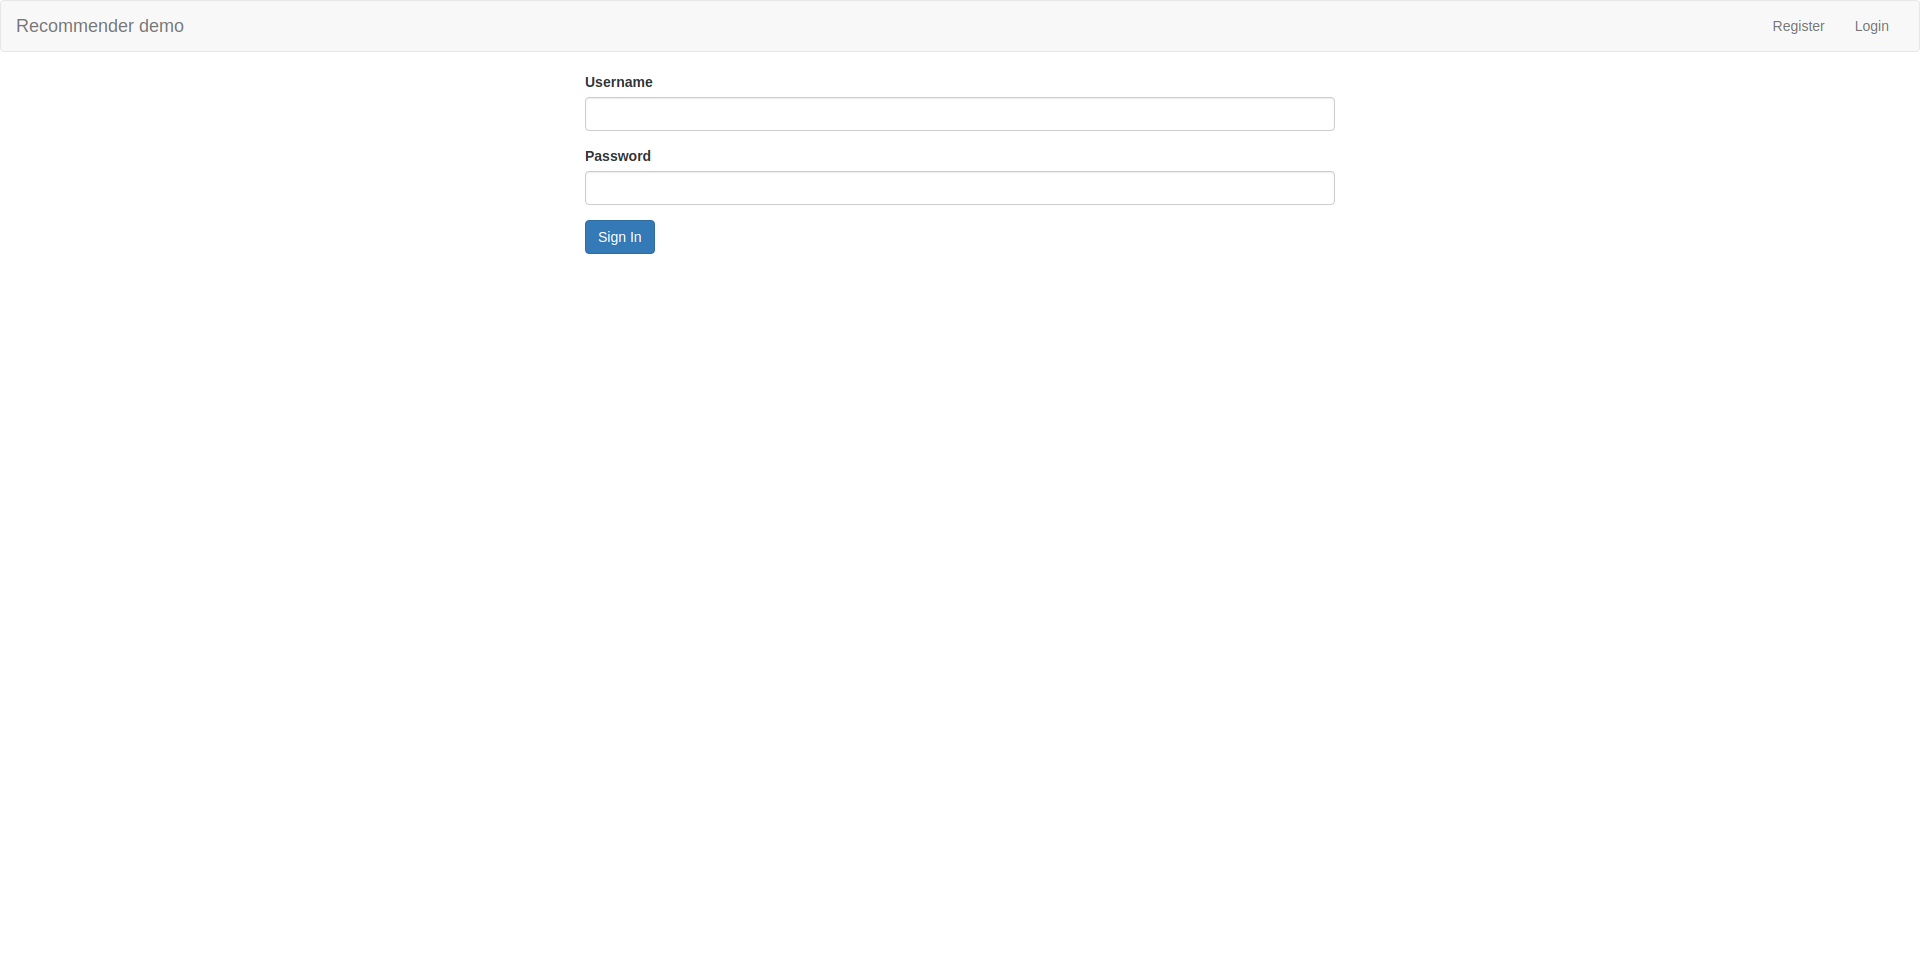
\includegraphics[width=1.0\textwidth]{./imgs/demo-preporucitelja-po-sadrzaju/tijek-rada/demo-login.png}
		\caption{Stranica za unos korisničkih podataka}
		\label{fg:demo_login}
	\end{center}
\end{figure}

Nakon što se uneseni podaci verificiraju korisnik se usmjerava na početnu stranicu gdje može pročitati kratke upute o korištenju aplikacije. Iste se upute u više detalja opisuju u nastavku.

Zajednička komponenta svim stranicama je navigacijski izbornik na vrhu stranice na kojem se nalaze poveznice: "Recommender demo", "Random Images", "Liked Images", "Recommended Images" te "Manage" izbornik s opcijom odjave "Log Out". "Recommender demo" poveznica je početnu stranicu, "Random Images" vodi na galeriju svih slika u sustavu, "Liked Images" poveznica je na galeriju slika koje je korisnik označio kao favorite dok je "Recommended Images" poveznica na galeriju slika koje sustav preporučuje na temelju korisničkih preferencija.

Prvi korak u korištenju aplikacije je odabir slika u galeriji nasumičnih slika korištenjem poveznice "Random Images"(Slika \ref{fg:demo_rand}). Ako korisnik odluči posjetiti neku od preostalih galerija prije nego što je označio ikakvu sliku, dobit će poruku upozorenja da sustav nije mogao obraditi njegov zahtjev. Jednom kad se galerija učitala, korisnik može početi pregledavati i označavati ponuđene slike. Sučelje se sastoji od dvije glavne komponente: trenutno razmatrane slike i podskupa slika galerije u obliku albuma. Album trenutnog pogleda na slike sustava pruža brzi pregled trenutne stranice slika. Gumbima "Previous Page" i "Next Page" korisnik može dohvaćati preostale stranice i postepeno pretražiti cijelu bazu slika. Gumbom "Refresh" korisnik može zatražiti osvježavanje trenutne stranice slika. Pritiskom na bilo koju od slika u albumu, slika se fokusira u gornjem pregledniku. Ispod fokusirane slike nalaze se tri gumba: gumb za pomak na prethodnu sliku albuma, gumb "Like" za dodavanje slike u favorite i gumb za pomak na iduću sliku albuma. Od korisnika se očekuje odabir najmanje jedne slike i pritisak na gumb "Like" prije prelaska u iduću fazu aplikacije.

\begin{figure}[!ht]
	\begin{center}
		\captionsetup{justification=centering}
		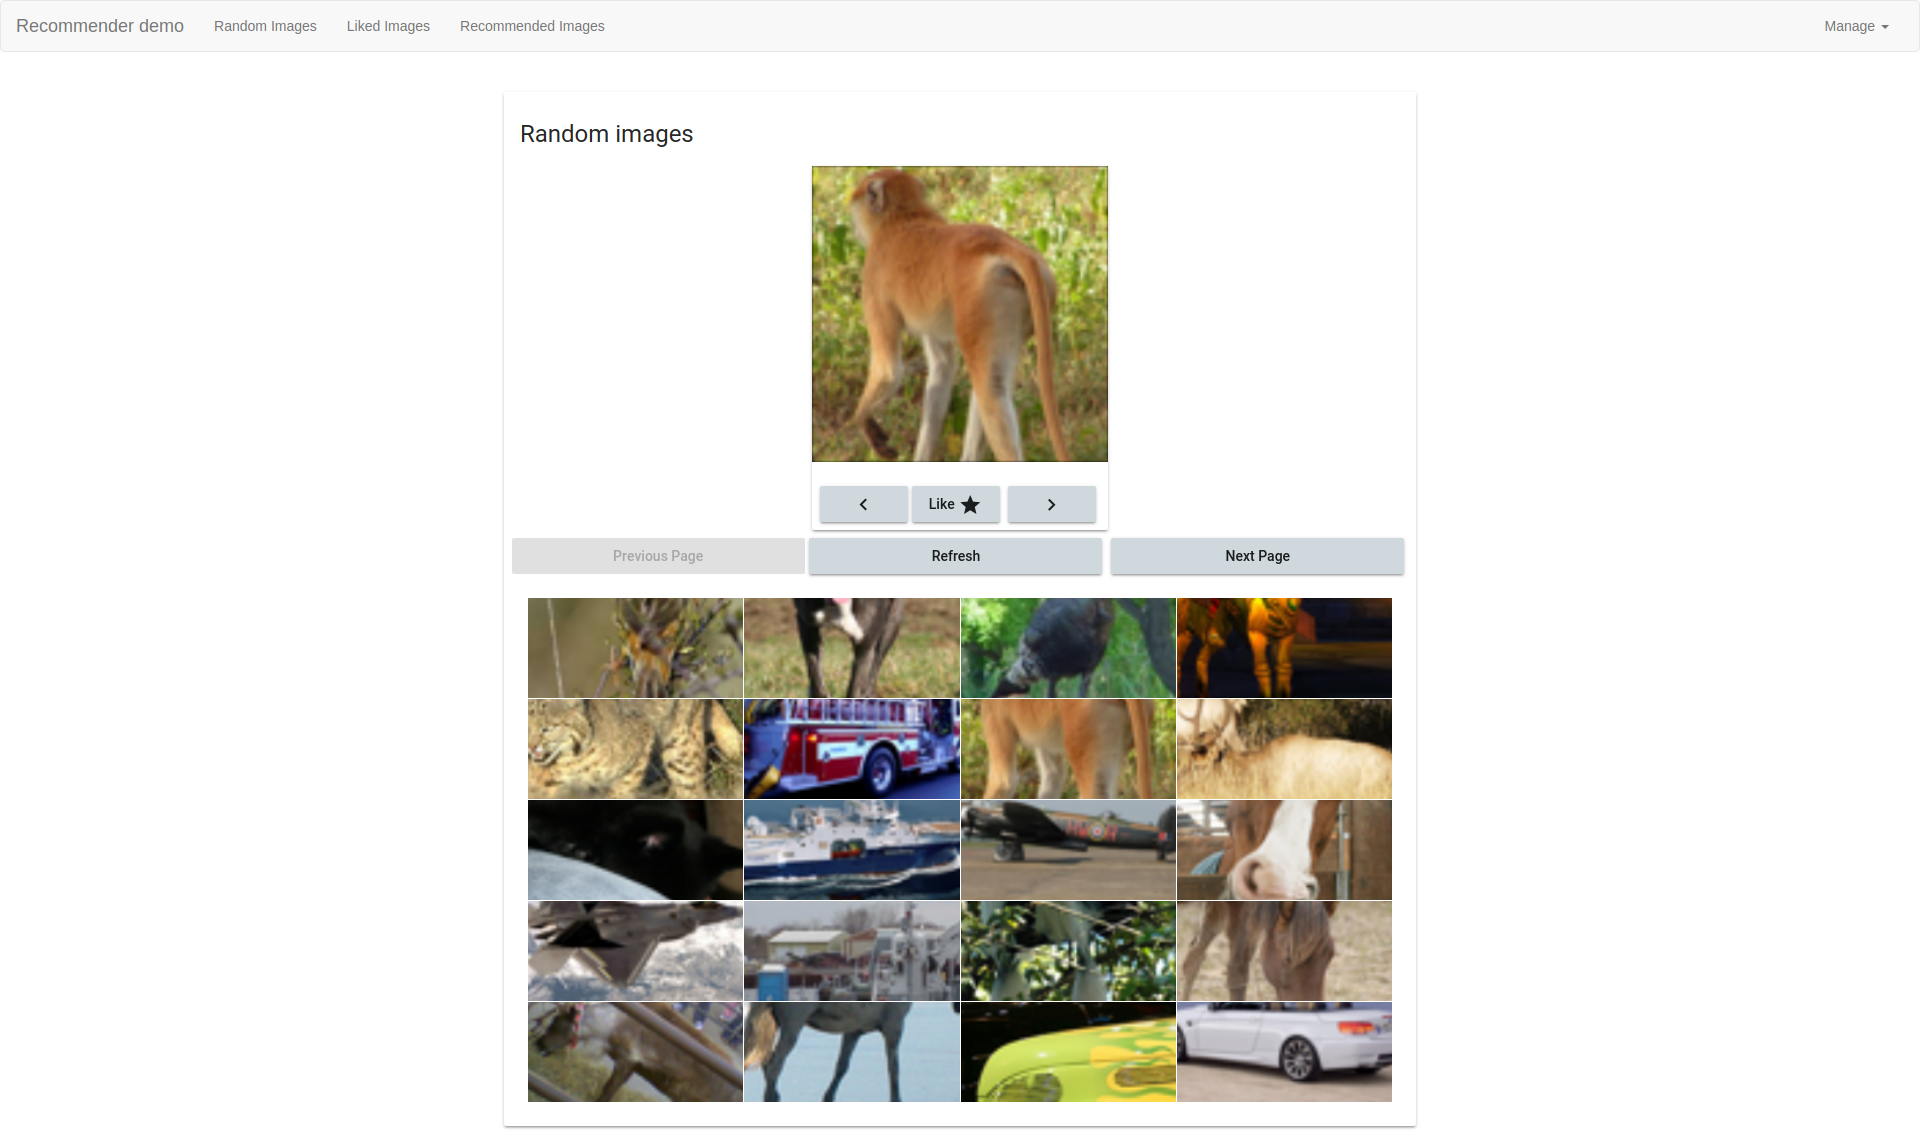
\includegraphics[width=1.0\textwidth]{./imgs/demo-preporucitelja-po-sadrzaju/tijek-rada/demo-rand.png}
		\caption{Galerija svih slika}
		\label{fg:demo_rand}
	\end{center}
\end{figure}


Nakon što je korisnik odabrao njemu interesantne slike, može ih još jednom pregledati pritiskom na poveznicu "Liked Images" (Slika \ref{fg:demo_liked}). Kroz ovaj pogled korisnik također može izbrisati neke od slika iz svojih favorita kako bi promotrio kako će to utjecati na preporuke sustava.

\begin{figure}[H]
	\begin{center}
		\captionsetup{justification=centering}
		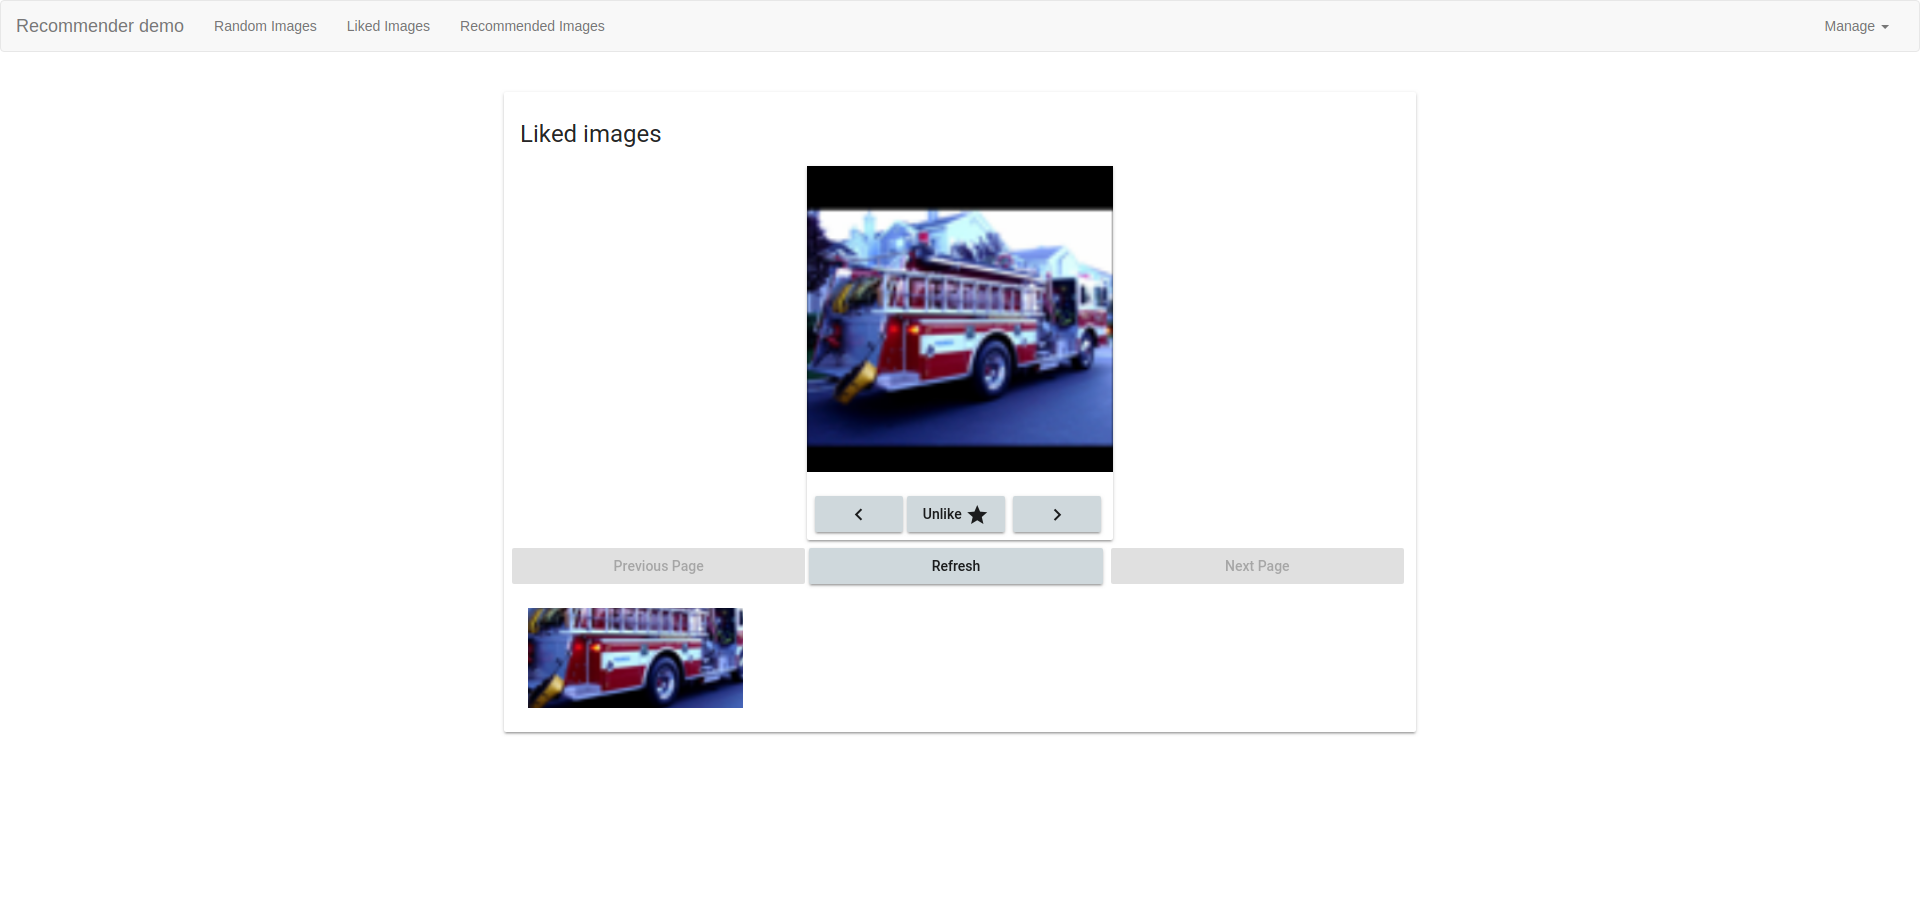
\includegraphics[width=1.0\textwidth]{./imgs/demo-preporucitelja-po-sadrzaju/tijek-rada/demo-liked.png}
		\caption{Galerija odabranih korisničkih slika}
		\label{fg:demo_liked}
	\end{center}
\end{figure}


Posljednja faza korištenja je pregledavanje preporučenih slika (Slika \ref{fg:demo_recommended}). Slično kao i u prethodnim pogledima, korisnik može dodavati slike u favorite, uz iznimku da sada pritiskom na "Refresh" gumb može brže zatražiti novi set preporuka prilagođen ažuriranom stanju preferencija. 

\begin{figure}[H]
	\begin{center}
		\captionsetup{justification=centering}
		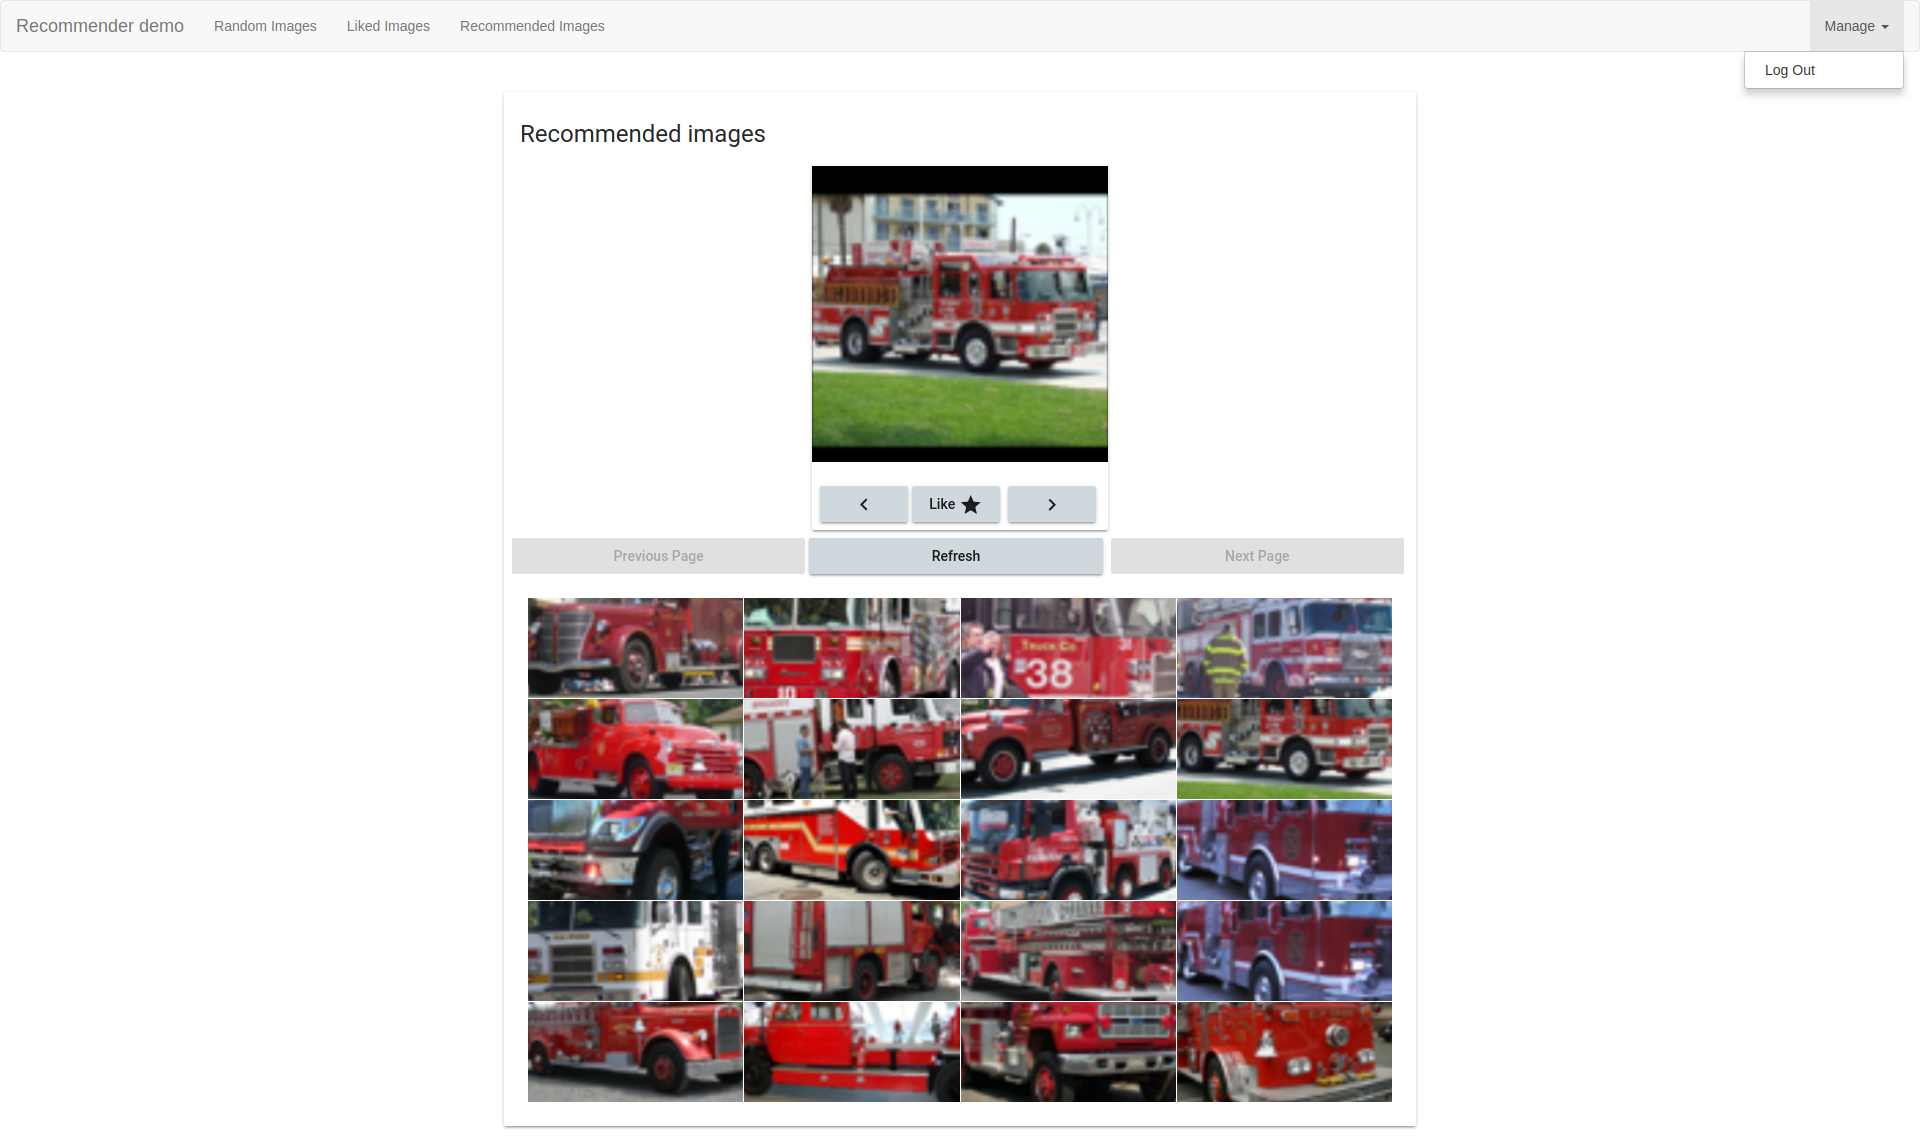
\includegraphics[width=1.0\textwidth]{./imgs/demo-preporucitelja-po-sadrzaju/tijek-rada/demo-reco.png}
		\caption{Galerija preporučenih slika}
		\label{fg:demo_recommended}
	\end{center}
\end{figure}


U nastavku slijedi par primjera odabranih ulaza i rezultirajućih preporuka. Sve rezultate moguće je reproducirati kroz \textit{web} stranicu. 

Odabirom prve slike ptice koja se nudi u albumu i odlaskom na pregled preporučenih slika možemo se uvjeriti da su dohvaćene slike uglavnom manjih ptica, ptica sličnih šara ili kombinacije navedenih svojstava (Slika \ref{fg:demo_bird}). 

\begin{figure*}[ht!]
	\begin{subfigure}[t]{0.24\textwidth}
		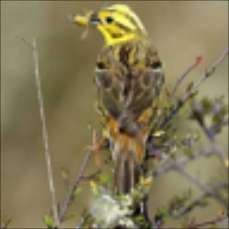
\includegraphics[width=\textwidth,height=\textwidth ]{./imgs/demo-preporucitelja-po-sadrzaju/tijek-rada/id@0.png}
	\end{subfigure}
	\rulesep
	\begin{subfigure}[t]{0.24\textwidth}
		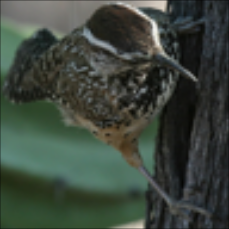
\includegraphics[width=\textwidth,height=\textwidth]{./imgs/demo-preporucitelja-po-sadrzaju/tijek-rada/id@182.png}
	\end{subfigure}
	\begin{subfigure}[t]{0.24\textwidth}
		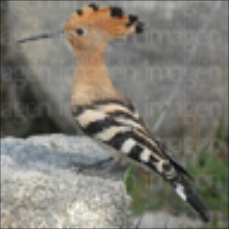
\includegraphics[width=\textwidth,height=\textwidth]{./imgs/demo-preporucitelja-po-sadrzaju/tijek-rada/id@1745.png}
	\end{subfigure}
	\begin{subfigure}[t]{0.24\textwidth}
		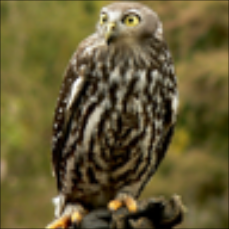
\includegraphics[width=\textwidth,height=\textwidth]{./imgs/demo-preporucitelja-po-sadrzaju/tijek-rada/id@2530.png}
	\end{subfigure}
	\caption{Primjer preporuka za sliku ptice}
	\label{fg:demo_bird}			
\end{figure*}


Ako sada izbrišemo preference i odaberemo drugačiju sliku poput purana na slici \ref{fg:demo_bird_v2}, preporuke se mijenjaju u slike većih ptica dugačkih vratova i nogu ili slika ptica slične posture poput našeg referentnog primjera. 

\begin{figure*}[ht!]
	\begin{subfigure}[t]{0.24\textwidth}
		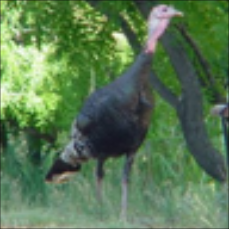
\includegraphics[width=\textwidth,height=\textwidth ]{./imgs/demo-preporucitelja-po-sadrzaju/tijek-rada/id@2.png}
	\end{subfigure}
	\rulesep
	\begin{subfigure}[t]{0.24\textwidth}
		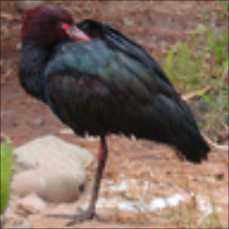
\includegraphics[width=\textwidth,height=\textwidth]{./imgs/demo-preporucitelja-po-sadrzaju/tijek-rada/id@148.png}
	\end{subfigure}
	\begin{subfigure}[t]{0.24\textwidth}
		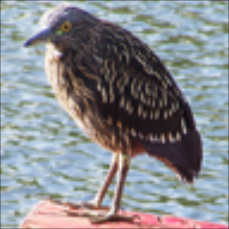
\includegraphics[width=\textwidth,height=\textwidth]{./imgs/demo-preporucitelja-po-sadrzaju/tijek-rada/id@4710.png}
	\end{subfigure}
	\begin{subfigure}[t]{0.24\textwidth}
		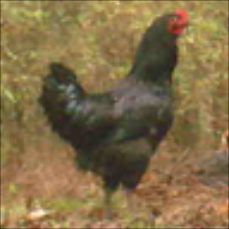
\includegraphics[width=\textwidth,height=\textwidth]{./imgs/demo-preporucitelja-po-sadrzaju/tijek-rada/id@3359.png}
	\end{subfigure}
	\caption{Primjer preporuka za sliku purana}
	\label{fg:demo_bird_v2}
		
\end{figure*}

\newpage

Provedimo još jedno testiranje ponovno uključujući sliku iz prvog eksperimenta(Slika \ref{fg:demo_bird_v3}). Sada možemo pronaći primjere koji su se pojavili i u prijašnjim upitima, ali i neke nove rezultate. Po završetku korištenja korisnik je dužan odjaviti se pritiskom na "Manage" te "Log Out" gumb u gornjem desnom uglu.


\begin{figure*}[ht!]
	\begin{subfigure}[t]{0.19\textwidth}
		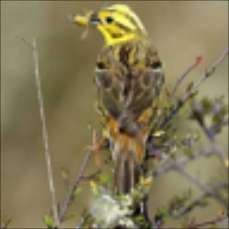
\includegraphics[width=\textwidth,height=\textwidth ]{./imgs/demo-preporucitelja-po-sadrzaju/tijek-rada/id@0.png}
	\end{subfigure}
	\begin{subfigure}[t]{0.19\textwidth}
		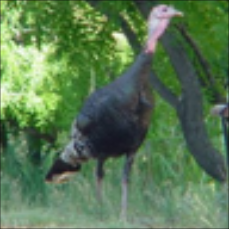
\includegraphics[width=\textwidth,height=\textwidth ]{./imgs/demo-preporucitelja-po-sadrzaju/tijek-rada/id@2.png}
	\end{subfigure}
	\rulesep
	\begin{subfigure}[t]{0.19\textwidth}
		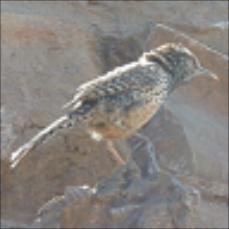
\includegraphics[width=\textwidth,height=\textwidth]{./imgs/demo-preporucitelja-po-sadrzaju/tijek-rada/id@4391.png}
	\end{subfigure}
	\begin{subfigure}[t]{0.19\textwidth}
		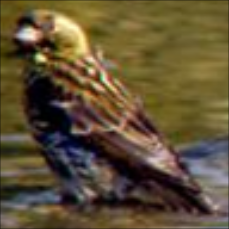
\includegraphics[width=\textwidth,height=\textwidth]{./imgs/demo-preporucitelja-po-sadrzaju/tijek-rada/id@3995.png}
	\end{subfigure}
	\begin{subfigure}[t]{0.19\textwidth}
		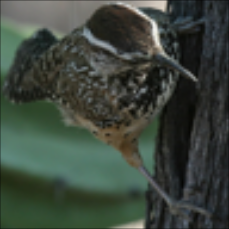
\includegraphics[width=\textwidth,height=\textwidth]{./imgs/demo-preporucitelja-po-sadrzaju/tijek-rada/id@182.png}
	\end{subfigure}
	\caption{Primjer preporuka za kombinaciju slika ptice i purana}
	\label{fg:demo_bird_v3}
		
\end{figure*}



\section{Implementacijski detalji}

Kao što je bilo naznačeno u poglavlju o paketima, implementacija \textit{web} poslužitelja oslanja se na dva programska jezika: Python i JavaScript. Poslužitelj \footnote{Kod poslužitelja dostupan je na \textit{Github} repozitoriju kojem možete pristupiti na linku \url{https://github.com/vribic/recommender-demo-api}.} je pisan u Python-u, oslanjajući se na \textit{Django} radno okruženje kako bi se podaci mogli dostavljati korisniku. Podaci aplikacije pohranjeni su u \textit{PostgreSQL} bazi podataka na samom serveru, dok se slike poslužuju s \textit{Amazon S3} servisa. Klijent \footnote{Kod klijenta dostupan je na \textit{Github} repozitoriju kojem možete pristupiti na linku \url{https://github.com/vribic/recommender-demo}.} je razvijen u standardnim \textit{web} tehnologijama \textit{HTML} (engl. \textit{HyperText Markup Language}), \textit{CSS} (engl. \textit{Cascading Style Sheets}) i JavaScript-u. Kako bi kod bio čim jednostavniji za razumijevanje i implementaciju, odabran je \textit{Angular 5} radni okvir za lakše oblikovanje komponenti klijenta. Po završetku razvoja aplikacija je postavljena na \textit{Heroku} platformu koja omogućuje izgradnju, pokretanje i upravljanje aplikacijama. Budući da implementacija same \textit{web} aplikacije nije bila predmet ovog rada zainteresirani čitatelji mogu dobiti više informacija posjećivanjem poveznica u podnožju stranice koje vode na repozitorije koda aplikacije.



%%%%%%%%%%%%%%%%%%%%%%%%%%%%%%%%%%%%%%%%%%%%%%%%%%%%%%%%%%%%%%%%%%%%%%%%%%%%%%%%%%%%%%%
%% CHAPTER
\chapter{Zaključak}

Rezultati su pokazali da je korištenjem dubokih modela moguće značajno reducirati reprezentaciju slika na nisko dimenzionalan vektor koji čuva njenu semantiku. Takva redukcija ostvaruje veliku uštedu korištene radne memorije i zbog svoje male dimenzionalnosti omogućuje brzu usporedbu i dohvat sličnih slika preko njihovih reduciranih reprezentacija. 

Budući da je u okviru ovog istraživanja korišten veliki i raznoliki skup podataka, kao i duboki modeli koji su trenirani na skupu podataka s drugačijom distribucijom od onoga na kojem su testirani, to ostavlja prostor za dodatne eksperimente za koje naši rezultati određuju donju granicu performansi. Razumno je pretpostaviti da bi se dodatna poboljšanja postigla kada bi se duboki model korišten za redukciju istrenirao na skupu podataka s istom distribucijom kao podaci koji će se koristiti u sustavu preporuke. Tako istrenirani model, omogućio bi izbor manje dimenzije reprezentativnog vektora čime bi se ostvarile još bolje performanse sustava u vidu preciznosti i memorijskih/vremenskih zahtjeva pretrage.

Daljnja istraživanja, kao i napreci u području dubokog učenja, ostavljaju mnogo prostora za detaljnije istraživanje dodatnih mogućnosti ekstrahiranja značajki.

%%%%%%%%%%%%%%%%%%%%%%%%%%%%%%%%%%%%%%%%%%%%%%%%%%%%%%%%%%%%%%%%%%%%%%%%%%%%%%%%%%%%%%%
\begin{sazetak}
		
	Slike čine veliki udio ukupnog volumena podataka na internetu. Zbog svojeg bogatog sadržaja koje pohranjuju, sve više suvremenih sustava ima potrebu za efikasnim upravljanjem i analizom slika. Stoga je fokus našeg rada na isprobavanju novih metoda iz područja analize slika kako bi se doskočilo novonastalim zahtjevima. Rad problemu pristupa kroz metodologiju dubokog učenja koja je posljednjih godinama privukla puno pažnje akademije i industrije pri radu s podacima bogatih informacijama, poput slika, teksta ili zvuka. Rezultat rada je sustav koji za dani set slika stvara nisko dimenzionalni zapis koji zadržava semantiku slike i pogodan je za usporedbu temeljem poznatih matematičkih metrika sličnosti. Pri testiranju različitih pristupa isprobani su predtrenirani modeli konvolucijskih neuronskih mreža, metode za redukciju dimenzionalnosti i metrike usporedbe. Kao primjer korištenja razvijanog sustava u sklopu ovog rada implementiran je sustav za preporučivanje slika na temelju korisničkih preferenci.
	
	\kljucnerijeci{Sustav za preporučivanje, Analiza slika, Duboko učenje, Konvolucijske neuronske mreže, Redukcija dimenzionalnosti, Pretraga velikih skupova podataka}
\end{sazetak}

\pagebreak

\engtitle{Extracting Image Features Using Deep Learning for Better Image Recommendation System Performance }
\begin{abstract}
	Images make up a large share of the total volume of data on the Internet. Because of their information rich content there exists a large demand for efficient handling and analysis of this data. Therefore our work focuses on testing novel methods from the field of image analysis in order to tackle the problems described. Due to recent advances in the field of deep learning there is an increasing interest from both the academia and industry in domains with huge datasets, such as images, text or audio. The outcome of this project is a functioning system which for a given set of images generates a low dimensional representation suitable for similarity search using existing mathematical tools. While designing the system we looked into different architectures and pretrained models of convolutional neural networks, methods for dimensionality reduction and similarity metrics. As a proof of concept we implemented an image recommendation system based on user preferences.
	
	\keywords{Recommendation systems, Image analysis, Deep learning, Convolutional neural networks, Dimensionality reduction, Information retrieval in big data}
\end{abstract}

%%%%%%%%%%%%%%%%%%%%%%%%%%%%%%%%%%%%%%%%%%%%%%%%%%%%%%%%%%%%%%%%%%%%%%%%%%%%%%%%%%%%%%%
%% DONE
\bibliography{references}
\bibliographystyle{unsrtnat}
\pagebreak

\end{document}